
\documentclass[10pt,conference,letterpaper]{ieee}
\usepackage{graphicx}
\usepackage{graphics}
\usepackage{colortbl}
\usepackage[noend]{algorithm2e}
\usepackage{amsmath}
\usepackage{algorithmic}
\usepackage[tight]{subfigure}
\usepackage{array}
\usepackage{url}
\usepackage{alltt}
\usepackage{paralist}
\usepackage{afterpage}
\usepackage{float}
%\usepackage[T1]{fontenc}
%\usepackage{times}


%\usepackage{caption}

\renewcommand{\textfraction}{0.07}	% allow minimal text w. figs


\def\compactify{\itemsep=0pt \topsep=0pt \partopsep=0pt \parsep=0pt}
\let\latexusecounter=\usecounter
\newenvironment{CompactItemize}
  {\def\usecounter{\compactify\latexusecounter}
   \begin{itemize}}
  {\end{itemize}\let\usecounter=\latexusecounter}
\newenvironment{CompactEnumerate}
  {\def\usecounter{\compactify\latexusecounter}
   \begin{enumerate}}
  {\end{enumerate}\let\usecounter=\latexusecounter}

\newcommand{\sys}{SubZero{}}
\newcommand{\red}[1]{\textcolor{red}{#1}}
\newcommand{\srm}[1]{\textcolor{red}{SRM: #1}}
\title{\sys{}: A Fine-Grained Lineage System for Scientific Databases}


\author{%
{Eugene Wu, Samuel Madden, Michael Stonebraker }
% add some space between author names and affils
\vspace{1.6mm}\\
\fontsize{10}{10}\selectfont\itshape
CSAIL, MIT\\
32 Vassar St, Cambridge, MA, USA 02139\\
\fontsize{9}{9}\selectfont\ttfamily\upshape
\{sirrice, madden, stonebraker\}@csail.mit.edu
}


%\restylefloat{figure}
%\restylefloat{table}
\setlength{\textfloatsep}{0pt}
\setlength{\floatsep}{0pt}
\setlength{\dbltextfloatsep}{10pt}
\setlength{\dblfloatsep}{0pt}
%\setlength{\abovecaptionskip}{0pt}
%\setlength{\belowcaptionskip}{0pt}

\begin{document}

\maketitle
\begin{abstract}


Data lineage is a key component of provenance that helps scientists  track and query
relationships between input and output data.  While current systems readily
support lineage relationships at the file or data array level, finer-grained
support at an array-cell level is impractical due to the lack of support
for user defined operators and the high runtime and storage overhead to store
such lineage.


We interviewed scientists in several domains to identify a set of common
semantics that can be leveraged to efficiently store fine-grained lineage.  We
use the insights to define lineage representations that efficiently capture
common locality properties in the lineage data, and a set of APIs so operator
developers can easily export lineage information from user defined operators.
Finally, we introduce two benchmarks derived from astronomy and genomics, and
show that our techniques can reduce lineage query costs by up to 10$\times$
while incuring substantially less impact on workflow runtime and storage.


%Provenance refers to the process of determining which inputs contributed
%to a particular output in a database query or scientific workflow.
%It is important in a number of debugging and exploratory development
%settings, and has been identified as a key requirement of next generation
%data management systems, particularly those focused on scientific use-cases
%where workflows can be very complex.
%
%In this paper, we present \sys{}, a provenance system for the SciDB
%scientific database system.  \sys{} builds on prior provenance systems
%by exploiting the semantics of scientific operations to efficiently
%encode provenance information, and provides an API for developers to
%record the provenance of their user-defined operators. \sys{} uses an
%optimization framework to select from several different methods of
%storing provenance, while respecting user-specified space and time
%constraints on the cost of recording provenance.  Two
%benchmarks derived from astronomy and genetics show that these
%optimizations make \sys{} up to 10$\times$ faster at executing a
%provenance query workload than a system that records fine-grained provenance
%between individual data items, while having substantially less impact
%on workflow runtime and requiring much less storage.



\end{abstract}


\section{Introduction}

Many scientific applications are naturally expressed as a workflow that
comprises a sequence of operations applied to raw input data to produce an
output dataset or visualization.  Like database queries, such workflows can be
quite complex, consisting up to hundreds of operations~\cite{lsst} whose
parameters or inputs vary from one run to another.  

Scientists record and query provenance -- metadata that describes the
processes, environment and relationships between input and output data arrays
-- to ascertain data quality, audit and debug workflows, and more generally
understand how the output data came to be. A key component of provenance, {\it
data lineage}, identifies how input data elements are related to output data
elements and is integral to debugging workflows.  For example, scientists need
to be able to work backward from the output to identify the sources of an error
given erroneous or suspicious output results.  Once the source of the error is
identified, the scientist will then often want to identify derived downstream
data elements that depend on the erroneous value so he can inspect and possibly
correct those outputs.  



In this paper, we describe the design of a fine-grained lineage tracking and
querying system for array-oriented scientific workflows.  We assume a data and
execution model similar to SciDB~\cite{scidb}.  We chose this because it
provides a closed execution environment  that can capture all of the lineage
information, and because it is specifically designed for scientific data
processing (scientists typically use RDBMSes to manage metadata and do data
processing outside of the database).  The system allows scientists to perform
exploratory workflow debugging by executing a series of {\it data lineage
queries} that walk backward to identify the specific cells in the input arrays
on which a given output cell depends and that walk forward to find the output
cells that a particular input cell influenced.  Such a system must manage input
to output relationships at a {\it fine-grained} array-cell level.

Prior work in data lineage tracking systems has largely been limited to
coarse-grained metadata tracking~\cite{taverna,genepattern}, which stores
relationships at the file or relational table level. {\it Fine-grained lineage}
tracks relationships at the array cell or tuple level.  The typical approach,
popularized by Trio~\cite{trio}, which we call {\it cell-level lineage},
eagerly materializes the identifiers of the input data records (e.g., tuples or
array cells) that each output record depends on, and  uses it to
directly answer backward lineage queries. An alternative, which we call {\it
black-box lineage}, simply records the input and output datasets and runtime
parameters of each operator as it is executed, and materializes the lineage at
lineage query time by re-running relevant operators in a tracing mode.

Unfortunately, both techniques are insufficient in scientific
applications for two reasons. First, scientific applications make heavy use of
user defined functions (UDFs), whose semantics are opaque to the lineage
system.  Existing approaches  conservatively assume that every output cell of a
UDF depends on every input cell, which limits the utility of a fine-grained
lineage system because it tracks a large amount of information without
providing any insight into which inputs actually contributed to a given output.
This necessitates proper APIs so that UDF designers can expose fine-grained
lineage information and operator semantics to the lineage system.

Second, neither black-box only nor cell-level only techniques are sufficient
for many applications. Scientific workflows consume data arrays that regularly
contain millions of cells, while generating complex relationships between
groups of input and output cells.    Storing cell-level lineage can avoid
re-running some computationally intensive operators (e.g., an image processing
operator that detects a small number of stars in telescope imagery), but needs
enormous amounts of storage if every output depends on every input (e.g., a
matrix sum operation) -- it may be preferable to recompute the lineage at
query time.  In addition, applications such as LSST\footnote{http://lsst.org}
are often subject to  limitations that only allow them to dedicate a
small percentage of storage to lineage operations.   Ideally, lineage 
systems would support a hybrid of the two approaches and take user constraints
into account when deciding which operators to store lineage for.


This paper seeks to address both challenges. We interviewed scientists from
several domains to understand their data processing workflows and  lineage
needs and used the results to design a science-oriented data lineage system.
We introduce {\it Region Lineage}, which exploits locality properties prevalent
in the scientific operators we encountered.  It addresses common relationships
between regions of input and output cells by storing grouped or summary
information rather than individual pairs of input and output cells. We
developed a lineage API that supports black-box lineage as well as {\it Region
Lineage}, which subsumes cell-level lineage.  Programmers can also specify
forward/backward {\it Mapping Functions} for an operator to directly
compute the forward/backward lineage solely from input/output cell coordinates
and operator arguments; we implemented these for many common matrix and
statistical functions.  We also developed a hybrid lineage storage
system that allows users to explicitly trade-off storage space for lineage
query performance using an optimization framework.  Finally, we introduce two
end-to-end scientific lineage benchmarks.

As mentioned earlier, the system prototype, \sys{}, is implemented in the
context of the SciDB model.  SciDB stores multi-dimensional arrays and executes
database queries composed of built-in and user-defined operators (UDFs) that
are compiled into workflows.  Given a set of user-specified storage
constraints, \sys{} uses an optimization framework to choose the optimal type
of lineage (black box, or one of several new types we propose) for each SciDB
operator that minimizes lineage query costs while respecting user storage
constraints.


A summary of our contributions include: 

\begin{CompactEnumerate}

\item The notion of {\it region lineage}, which \sys{} uses to efficiently
    store and query lineage data from scientific applications.  We also
    introduce several efficient representations and encoding schemes that each
    have different overhead and query performance trade offs.

\item A {\it lineage API} that operator developers can use to expose lineage
    from user defined operators, including the specification of {\it mapping
    functions} for many of the built in SciDB operators.

\item A {\it unified storage model} for mapping functions, region and
    cell-level lineage, and black-box lineage.

\item An {\it optimization framework} which picks an optimal mixture of
    black-box and region lineage  to maximize query
    performance within user defined constraints.

\item A performance evaluation of our approach on end-to-end astronomy and
    genomics benchmarks.  The astronomy benchmark, which is computationally
    intensive but exhibits high locality, benefits from efficient
    representations.  Compared to cell-level and black-box lineage, \sys{}
    reduces storage overhead by nearly 70$\times$ and speeds query performance
    by almost 255$\times$.  The genomics benchmark highlights the need for, and
    benefits of, using an optimizer to pick the storage layout, which improves
    query performance by 2--3$\times$ while staying within user constraints.
    

\end{CompactEnumerate}

The next section  describes our motivating use cases in more detail.  It is
followed by a high level system architecture and details of the rest of the
system.














\section{Use Cases}
\label{s:usecases}


We developed two benchmark applications after discussions with environmental
scientists, astronomists, and geneticists.  The first is an image processing
benchmark developed with scientists at the Large Synoptic Survey Telescope
(LSST) project.  It is very similar to environmental science requirements, so
they are combined together. The second was developed with geneticists at the
Broad Institute\footnote{\url{http://www.broadinstitute.org/}}.  Each benchmark
consists of a workflow description, a dataset, and lineage queries.  We used
the benchmarks to design the optimizations described in the paper.   This
section will briefly describe each benchmark's scientific application, the
types of desired lineage queries, and application-specific insights.


\subsection{Astronomy} 
\label{s:ucastro}



The Large Synaptic Survey Telescope (LSST) is a wide angle telescope slated to
begin operation in Fall 2015.  A key challenge in processing telescope images is
filtering out high energy particles (cosmic rays) that create abnormally bright
pixels in the resulting image, which can be mistaken for stars.  The telescope
compensates  by taking two consecutive pictures of the same piece of the sky
and removing the cosmic rays in software.  The LSST image processing workflow
(Figure \ref{f:lsstworkflow}) takes two images as input and outputs an
annotated image that labels each pixel with the celestial body it belongs to.
It first cleans and detects cosmic rays in each image separately, then creates
a single composite, cosmic-ray-free, image that is used to detect celestial
bodies.  There are 22 SciDB built-in operators (blue solid boxes) that perform
common matrix operations, such as convolution, and four UDFs (red dotted boxes
labeled A-D).  The UDFs A and B output cosmic-ray masks for each of the images.
After the images are subsequently merged, C removes cosmic-rays from the
composite image, and D detects stars from the cleaned image.  


The LSST scientists are interested in three types of queries.  The first picks
a star in the output image and traces the lineage back to the initial
input image to detect bad input pixels.  The latter two queries select a
region of output (or input) pixels and trace the pixels backward (or forward)
through a subset of the workflow to identify a single faulty operator.  
%These queries only partially trace through the workflow because it is often a
%single operator that is the obvious point of error.  
As an example, suppose the operator that computes the mean brightness of the
image  generated an anomalously high value due to a few bad pixel, which led to
further mis-calculations.  The astronomer might work backward from those
calculations, identify the input pixels that contributed to them, and filter out
those pixels that appear excessively bright.

Both the LSST and environmental scientists described workloads where the majority
of the data processing code computes output pixels using input pixels within a
small distance from the corresponding coordinate of the output pixel.  These
regions may be constant, pre-defined values, or easily computed from a small
amount of additional metadata.  For example, a pixel in the mask produced by
cosmic ray detection ($CRD$) is set if the related input pixel is a cosmic ray,
and depends on neighboring input cells within 3 pixels.  Otherwise, it only
depends on the related input pixel.  They also felt that it is sufficient for lineage queries
to return a superset of the exact lineage.  Although we do not take
advantage of this insight, this suggests future work in lossy compression
techniques.




\begin{figure}[h] \centerline{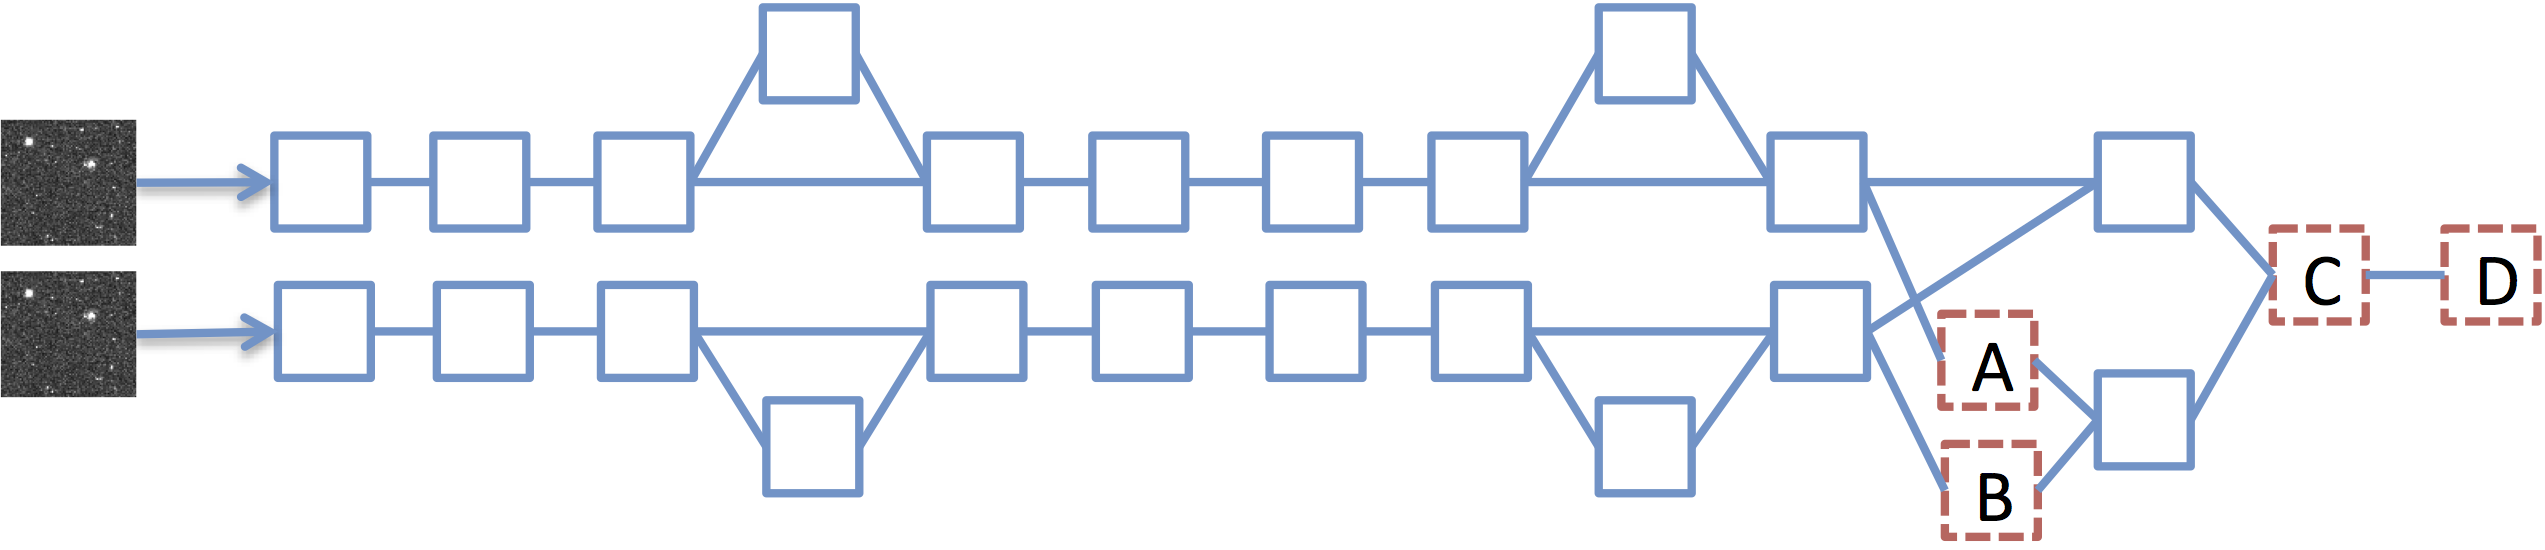
\includegraphics[width=3.3in,natwidth=8.49in,natheight=1.84in]{figures/lsst.png}}
\caption{Summary diagram of LSST workflow.  Each solid rectangle is a SciDB
native operator while the red dotted rectangles are UDFs.}
\label{f:lsstworkflow} \end{figure}
 













\subsection{Genomics Prediction} \label{s:ucgenomics}


We have also been working with researchers at the Broad Institute on a genomics
benchmark related to predicting recurrences of medulloblastoma in patients.
Medulloblastoma is a form of cancer that spawns brain tumors that spread
through the cerebrospinal fluid.  Pablo et.~al~\cite{pablo} have identified a
set of patient features that help predict relapse in medulloblastoma patients
that have been treated.  The features include histology, gene expression levels,  and the existence of genetic abnormalities.  The
workflow (Figure \ref{f:genomicsworkflow}) is a two-step process that first
takes a training patient-feature matrix and outputs a Bayesian model.  Then it
uses the model to predict relapse in a test patient-feature matrix.  The model
computes how much each feature value contributes to the likelihood of patient
relapse.  The ten built-in operators (solid blue boxes) are simple matrix
transformations.  The remaining UDFs extract a subset of the input arrays
(E,G), compute the model (F), and predict the relapse probability (H).

The model is designed to be used by clinicians through a visualization that
generates lineage queries.  The first query picks a relapse prediction and traces its
lineage back to the training matrix to find supporting input data. The second
query picks a feature  from the model and traces it back to the training
matrix to find the contributing input values.  The third query points at a set
of training values and traces them forward to the model, while the last query
traces them to the end of the workflow to find the predictions they affected.

The genomics benchmark can devote up-front storage and runtime overhead to
ensure fast  query execution because it is an interactive visualization.
Although this is application specific, it suggests that scientific applications
have a wide range of storage and runtime overhead constraints.



\begin{figure}[h] \centerline{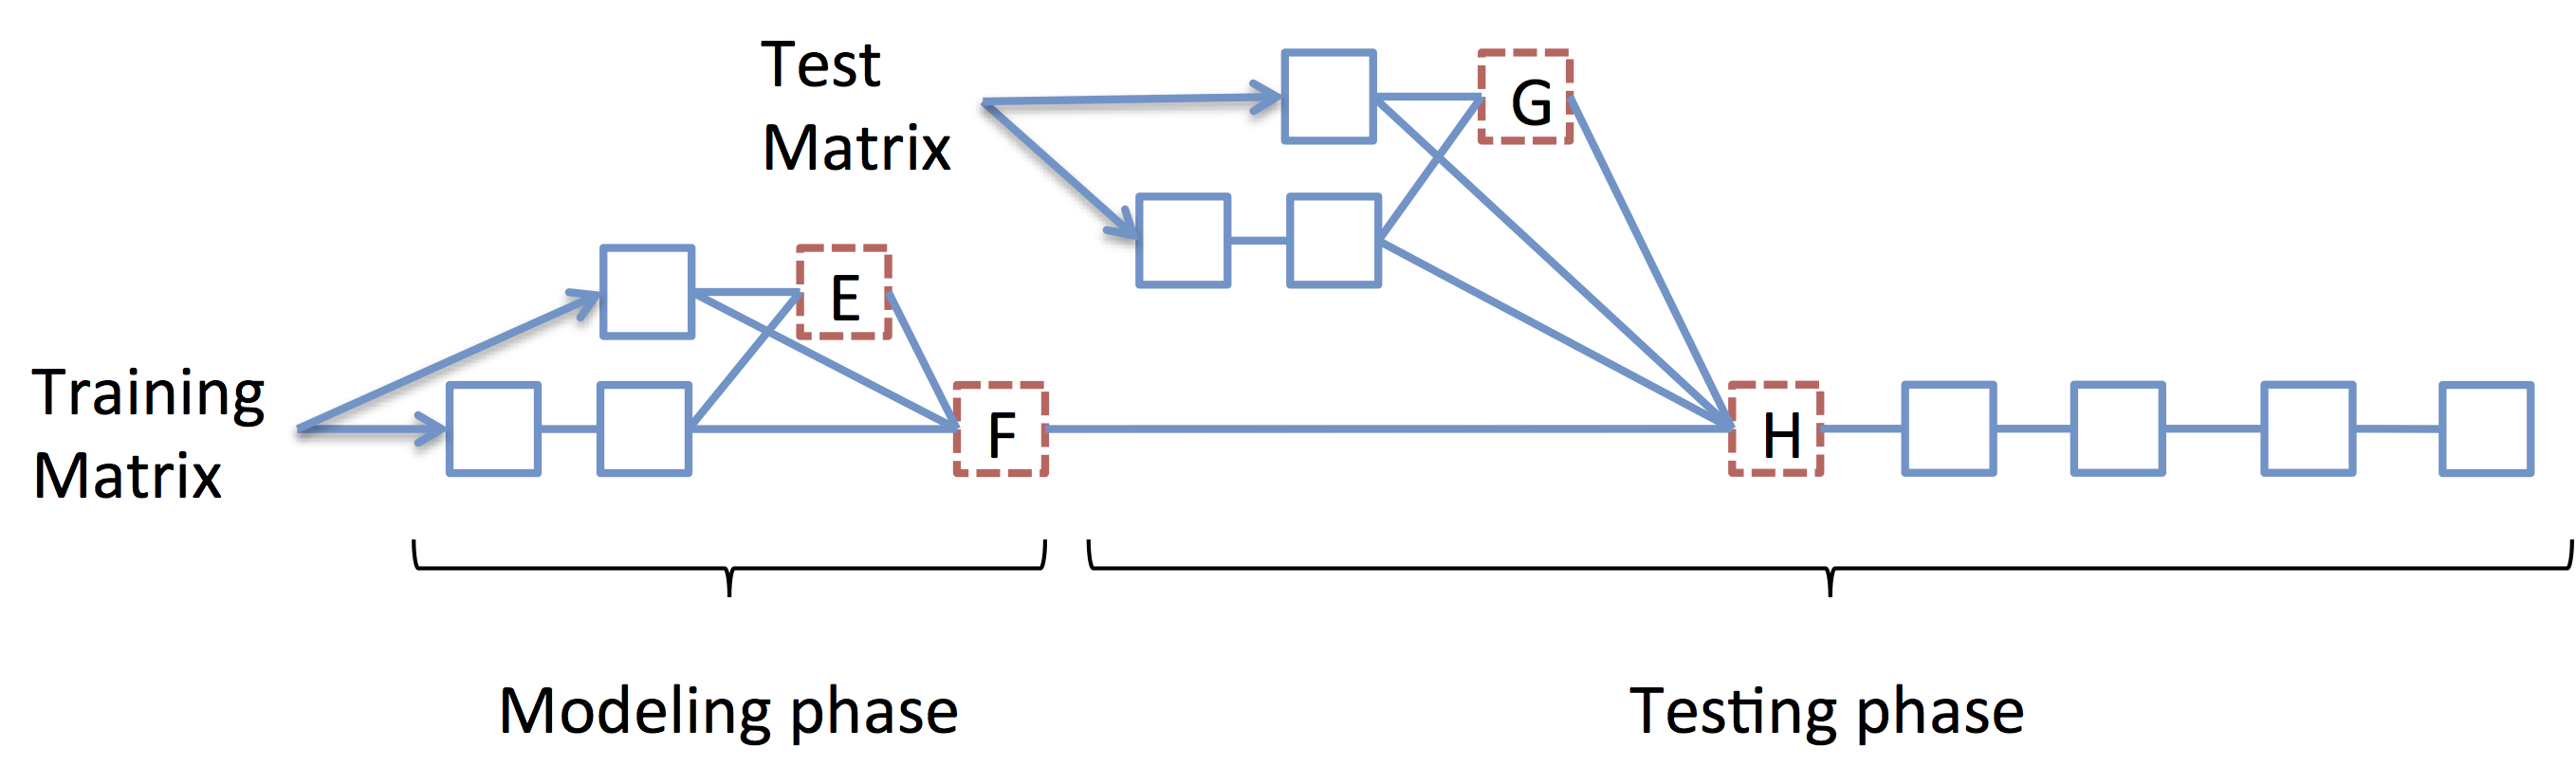
\includegraphics[width=3.3in,natwidth=9.06in,natheight=2.7in]{figures/genomics.png}}
\caption{Simplified diagram of genomics workflow.  Each solid rectangle is a
SciDB native operator while the red dotted rectangles are UDFs.}
\label{f:genomicsworkflow} \end{figure}




\section{Architecture}
\label{s:arch}



\begin{figure}[h!]
\begin{center}
   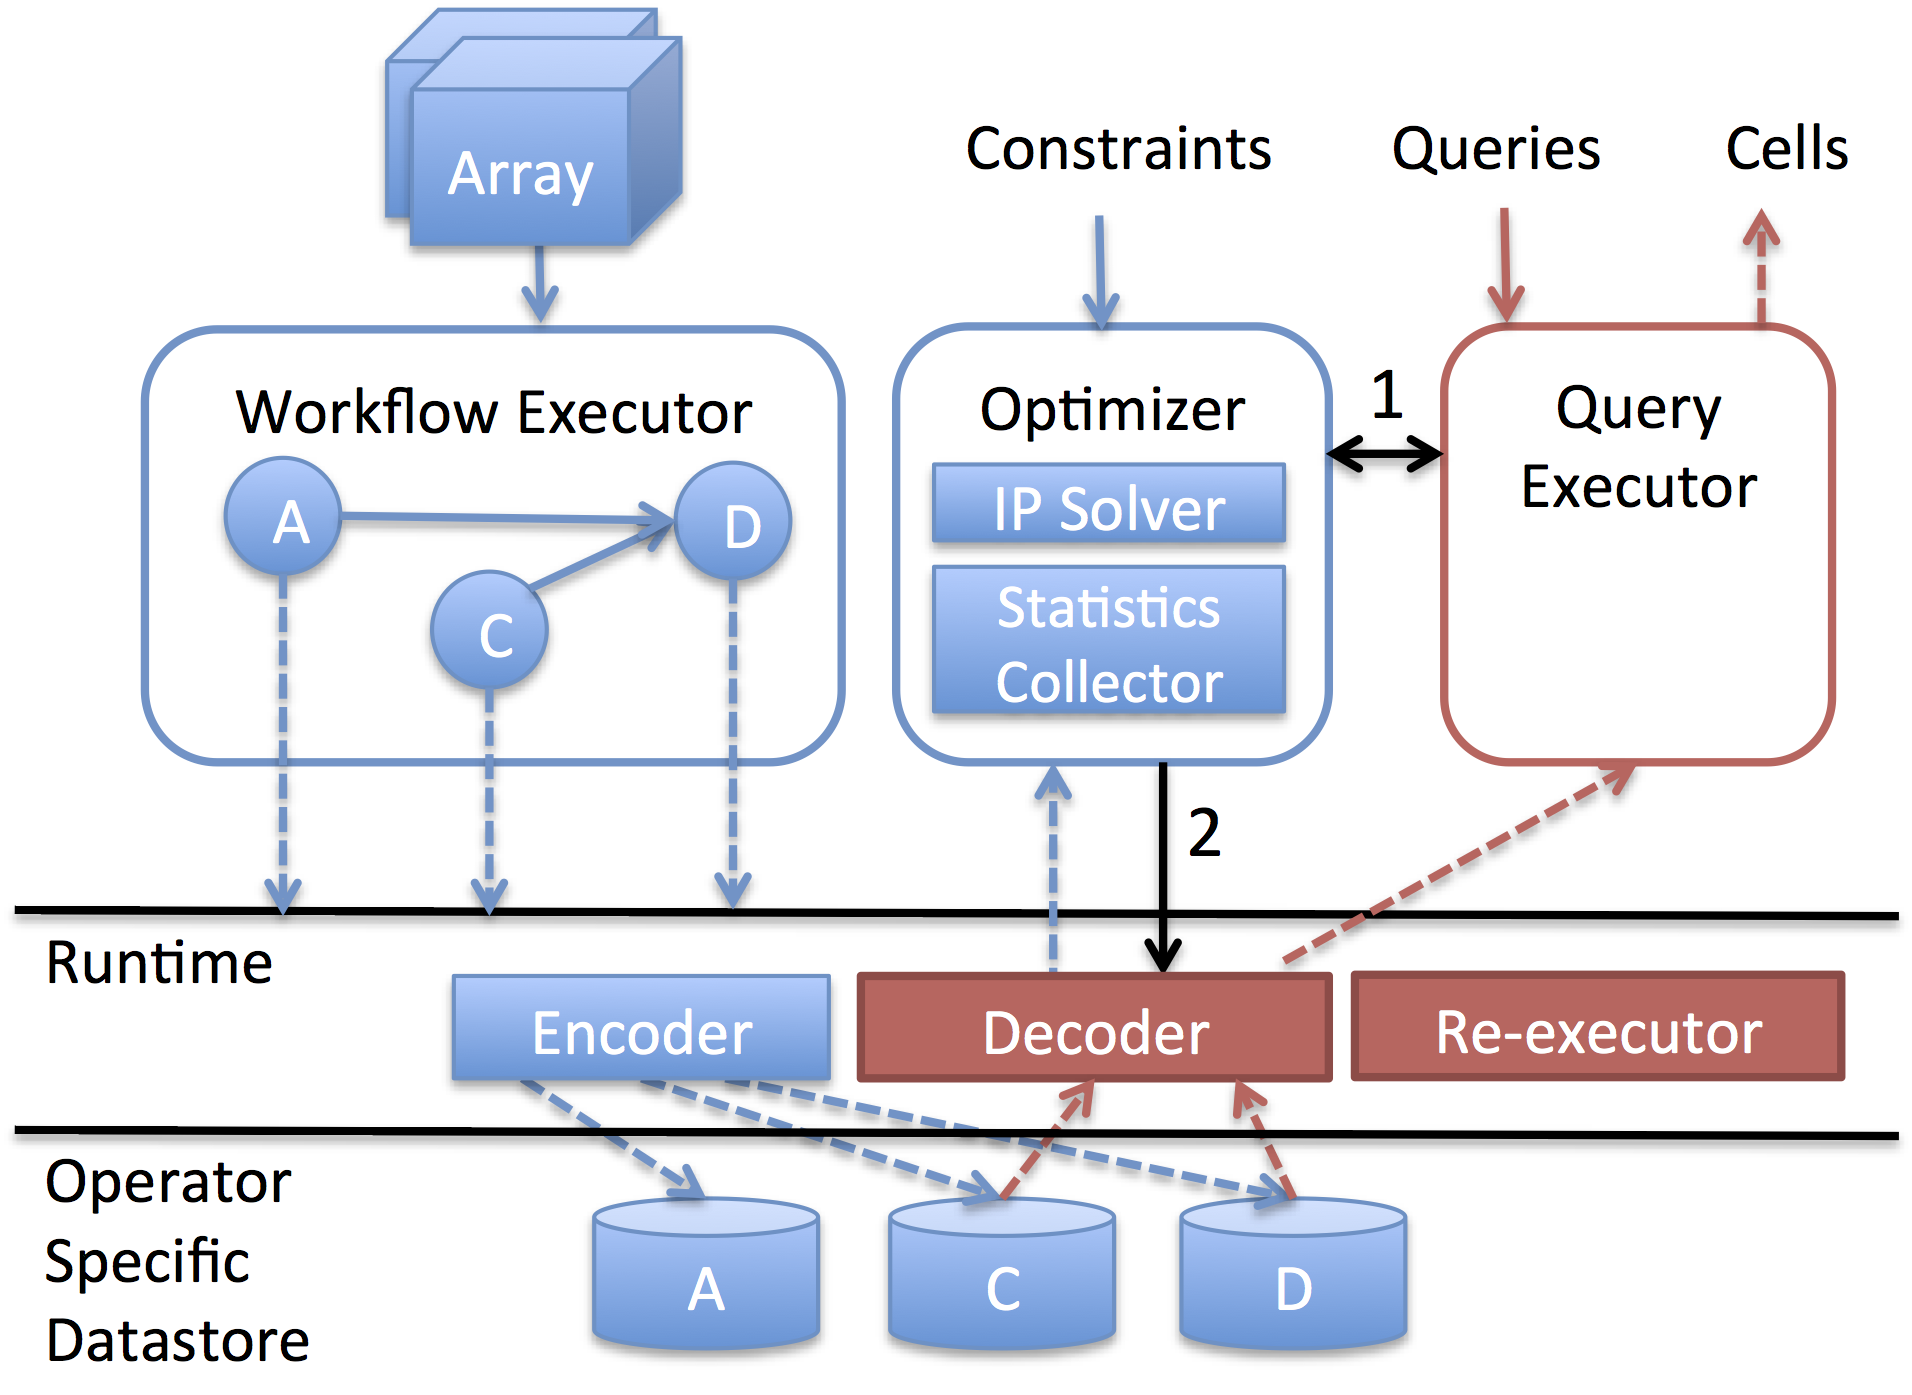
\includegraphics[width=2.9in,natwidth=6.38in,natheight=4.66in]{figures/arch.png}
\caption{The \sys{} architecture.  }
\vspace{-.1in} 
\label{f:arch}
\end{center}
\end{figure}

\sys{} records and stores lineage data at workflow runtime and uses it
to efficiently execute lineage queries.  The input to \sys{} is a
workflow specification (the graph in {\it Workflow Executor}),
constraints on the amount of storage that can be devoted to lineage
tracking, and a sample lineage query workload that the user expects to run.  \sys{} optimally decides
the type of lineage that each operator in the workflow will
generate ( the {\it lineage strategy}) in order to maximize the
performance of the query workload performance.


Figure \ref{f:arch} shows the system architecture.  The solid and
dashed arrows indicate the control and data flow, respectively.  Users
interact with \sys{} by defining and executing workflows ({\it
  Workflow Executor}), specifying constraints to the {\it Optimizer},
and running lineage queries ({\it Query Executor}).  The operators
in the workflow specify a list of the types of lineage
(described in Section~\ref{s:storagemodel}) that each operator can
generate, which defines the set of optimization possibilities.  

Each
operator initially generates black-box lineage (i.e., just records the names of the inputs it processes) but over time
changes its strategy through optimization.  As operators 
process data, they send lineage to the {\it
  Runtime}, which uses
the {\it Encoder} to serialize the lineage before writing it to
{\it Operator Specific Datastores}.  The {\it Runtime} may also send
lineage and other statistics to the {\it Optimizer}, which
calculates  statistics such as the amount of
lineage that each operator generates.  \sys{} periodically runs the
{\it Optimizer}, which uses an {\it Integer Programming Solver} to compute
the new lineage strategy.  On the right side, the {\it Query
  Executor} compiles lineage queries into query plans that join the
query with lineage data.  The {\it Executor} requests lineage
from the {\it Runtime}, which  reads and decodes  stored
lineage, uses the {\it Re-executor} to re-run the operators, and
 sends statistics (e.g., query fanout and
fanin) to the optimizer to refine future optimizations.

Given this  overview, we now describe the data model and structure of lineage
queries (Section~\ref{s:datamodel}), the different types of lineage the system
can record (Section~\ref{s:storagemodel}), the functionality of the {\it
Runtime}, {\it Encoder}, and {\it Query Executor} (Section~\ref{s:imp}), and finally
the optimizer in Section~\ref{s:optimizer}. 


\section{Data, Lineage and Query Model}
\label{s:datamodel}

In this section, we describe the representation and notation of lineage 
data and queries in \sys{}.

\sys{} is designed to work with a workflow executor system that applies a fixed
sequence of operators to some set of inputs.  Each operator operates
on one or more input objects (e.g., tables or arrays), and produces a
single output object.  Formally, we say an operator $P$ takes as input
$n$ objects, $I_P^1,...,I_P^n$, and outputs a single object, $O_P$.

Multiple operators are composed together to form a workflow, described by a
workflow specification, which is a directed acyclic graph $W = (N, E)$, where
$N$ is the set of operators, and $e = (O^P, I^{P'}_i) \in E$ specifies that the
output of $P$ forms the {\it i'th} input to the operator $P'$.  An instance of
$W$, $W_j$, executes the workflow on a specific dataset. Each operator runs
when all of its inputs are available.

The data follows the SciDB data model, which processes multi-dimensional
arrays.  A combination of values along each dimension, termed a {\it
coordinate}, uniquely identifies a cell.  Each cell in an array has the same
schema, and consists of one or more named, typed fields.  SciDB is ``no
overwrite,'' meaning that intermediate results produced as the output of an
operator are always stored persistently, and each update to an object creates a
new, persistent version.  \sys{} stores lineage information
with each version to speed up lineage queries. 


Our notion of backward lineage is defined as a subset of the inputs that will
reproduce the same output value  if the operator is re-run on its lineage.  For
example, the lineage of an output cell of Matrix Multiply are all cells of the
corresponding row and column in the input arrays -- even if some are empty.
Forward lineage is defined as a subset, $C$, of the outputs such that the
backward lineage of $C$ contains the input cells.  The exact semantics for UDFs
are ulitmately controlled by the developer.

%This definition is consistent with other provenance models that assume
%all-to-all relationships across UDFs.  While this is sufficient for the
%applications we encountered, enforcing stricter semantics in lineage systems
%that support UDFs is an important subject of future work.




%Finally, we define the $fanout$($fanin$) of an operator as the average number
%of output(input) cells that are derived from each input(output) cell. 

%Black-box lineage only stores references to the input and output arrays as
%each operator is executed.  
\sys{} supports three types of lineage: {\it black box},  {\it cell-level}, and {\it region}
lineage.
As a workflow executes, lineage is generated on an operator-by-operator basis,
depending on the types of lineage that each operator is instrumented to support
and the materialization decisions made by the optimizer.  We have instrumented
SciDB's built-in operators to generate lineage mappings from inputs to
outputs and provide an API for
UDF designers to expose these relationships.  If the API is not used, then \sys{}
assumes an all-to-all relationship between the cells of the input arrays and
cells of the output array.



\paragraph{Black-box lineage}\sys{} does not require additional resources to store black-box lineage because, like SciDB,
our workflow executor records intermediate results as well as input and output array versions
as peristent, named objects. These are sufficient to re-run any previously executed
operator from any point in the workflow.

%Black box lineage allows any output cell to be recreated by re-running the
%operator with the original inputs. % and filtering the lineage that is
%generated.

\paragraph{Cell-level lineage} Cell-level lineage models the relationships
between an output cell and each input cell that generated it \footnote{Although
    we model and refer to lineage as a mapping between input and output cells,
    in the \sys{} implementation we store these mappings as references to
physical cell coordinates.} as a set of pairs of input and output cells:
{\footnotesize $$\{(out,in) | out \in O_P \wedge in \in \cup_{i\in [1,n]} I_P^i
\}$$ } Here, $out \in O_P$ means that $out$ is a single cell contained in the
output array $O_P$.  $in$ refers to a single cell in one of the input arrays.

\paragraph{Region lineage} Region lineage 
models lineage as a set of {\it region pairs}.  Each region pair describes an
all-to-all lineage relationship between a set of output cells, $outcells$, and
a set of input cells, $incells_i$, in each input array, $I_P^i$: 
{\footnotesize
    $$\{(outcells,incells_1,...,incells_n) | outcells \subseteq O_P
    \wedge incells_i \subseteq I_P^i\}$$ }
Region lineage is more than a short hand; scientific applications often exhibit
locality and generate multiple output cells from the same set of input cells,
which can be represented by a single region pair.  For example, the LSST star
detection operator finds clusters of adjacent bright pixels and generates an
array that labels each pixel with the star that it belongs to.  Every output
pixel labeled {\it Star X} depends on all of the input pixels in the {\it Star
X} region.  Automatically tracking such relationships at the cell level  is
particularly expensive, so region lineage is a generalization of cell-level
lineage that makes this relationship explicit.  For this reason, later sections
will exclusively discuss region pairs.




%\subsection{Query Model}

Users execute a lineage query by specifying the coordinates of
an initial set of query cells, $C$, in a starting array, and a path of
operators $(P_1 \ldots P_m)$  to trace through the workflow:
{\footnotesize
    $$R = execute\_query(C, ((P_1, idx_1),..., (P_m, idx_m)))$$
}
Here, the indexes ($idx_1 \ldots idx_m$) are used to disambiguate which input
of a multi-input operator that the query path traverses.  

Depending on the order of operators in the query path, \sys{} recognizes the
query as a {\it forward lineage query} or {\it backward lineage query}.  A {\it
forward lineage query} defines a path from some ancestor operator $P_1$ to some
descendent operator $P_m$.  The output of an operator $P_{i-1}$ is  the
$idx_i$'th input of the next operator, $P_i$.  The query cells $C$ are a
subset of $P_1$'s $idx_1$'th input array, $C \subseteq I_{P_1}^{idx_1}$.

A {\it backward lineage query} reverses this process, defining a path from some
descendent operator, $P_1$ that terminates at some ancestor operator, $P_m$.
The output of an operator, $P_{i+1}$ is the $idx_i$'th input of the previous
operator, $P_i$, and the query cells $C$ are a subset of $P_1$'s output array,
$C \subseteq O_{P_1}$.  
The query results are the coordinates of the cells $R \subseteq O_{P_m}$ or $R
\subseteq I_{P_m}^{idx_m}$, for forward and backward queries, respectively.



%It is also used when the output of an operator is used
%as multiple inputs to
%the same operator (e.g., self-join).  









\section{Lineage API and Storage Model}
\label{s:storagemodel}

\sys{} allows developers to write operators that efficiently represent and
store  lineage.  This section describes several modes of region lineage, and an
API that UDF developers can use to generate lineage from within the operators.  We
also introduce a mechanism to control the modes of lineage that an operator
generates.  Finally, we describe how \sys{} re-executes black-box operators
during a lineage query.  Table \ref{t:api} summarizes the API calls and
operator methods that are introduced in this section.

Before describing the different lineage storage methods, we illustrate the
basic structure of an operator:

{\footnotesize
\begin{alltt}
class OpName:
   def run(input-1,...,input-n,cur_modes):
      /* Process the inputs, emit the output */
      /* Record lineage modes specified
         in cur_modes */
    def supported_modes():
      /* Return the lineage modes the
         operator supports */
\end{alltt}
}

Each operator implements a {\it run()} method, which is called when inputs are
available to be processed.  It is passed a list of lineage modes it should
output in the {\it cur\_modes} argument; it writes out lineage data using
the {\it lwrite()} method described below.  The developer specifies the modes
that the operator supports (and that the runtime will consider) by overriding
the {\it supported\_modes()} method.  If the developer does not override {\it
supported\_modes()}, \sys{} assumes an all-to-all relationship between the
inputs and outputs.  Otherwise, the operator automatically supports black-box
lineage.



\begin{table}[t!]
\vspace{-.2in}
\advance\leftskip-.3in
\footnotesize
\caption{Runtime and operator methods}
%\begin{center}
  \begin{tabular}{ | l | l  | }
    \hline
    {\bf API Method} & {\bf Description} \\ \hline \hline
    \multicolumn{2}{|c|}{\bf System API Calls} \\ \hline
    lwrite(outcells, ${\rm incells_1}$, ...,$ {\rm incells_n}$) & API
    to store lineage relationship.   \\ \hline
    lwrite(outcells, payload) & API to store small binary payload\\
                              &instead of input cells.  Called by \\
			      &payload operators.  \\ \hline
    \multicolumn{2}{|c|}{\bf Operator Methods} \\ \hline
    run(input-1,...,input-n,cur\_modes)
                              & Execute the operator, generating \\
			      & lineage types in cur\_modes $\subseteq \{Full,$\\
			      &$Map, Pay, Comp, Blackbox\}$  \\ \hline

    ${\rm map_b}$(outcell, i) & Computes the input cells in ${\rm input_i}$\\
                              &that contribute to ${\rm outcell}$.\\ \hline
    ${\rm map_f}$(incell, i) & Computes the output cells that depend\\
                             &on ${\rm incell} \in {\rm input_i}$. \\ \hline
    ${\rm map_p}$(outcell, payload, i)
                             & Computes the input cells in  ${\rm input_i}$ \\
			     &that contribute to ${\rm outcell}$, has access \\
			     &to ${\rm payload}$. \\ \hline
    supported\_modes()  &  Returns the lineage modes $C \subseteq \{Full,$\\
                        &$Map, Pay, Comp, Blackbox\}$ \\
    &that the operator can generate. \\ \hline


\end{tabular}
%\end{center}
\label{t:api}
\end{table}



For ease of explanation, this section is described in the context of
the LSST operator $CRD$ (cosmic ray detection, depicted as A and B in
Figure~\ref{f:lsstworkflow}) that finds pixels containing cosmic rays
in a single image, and outputs an array of the same size.  If a pixel
contains a cosmic ray, the corresponding cell in the output is set to
$1$, and the output cell depends on the 49 neighboring pixels within a
3 pixel radius.  Otherwise the output cell is set to $0$, and only
depends on the corresponding input pixel.  A region pair is denoted
($outcells$, $incells$).



\subsection{Lineage Modes}

\sys{} supports four modes of region lineage ({\it Full, Map, Pay, Comp}), and
one mode  of black-box lineage ({\it Blackbox}).  {\it cur\_modes} is set to
{\it Blackbox} when the operator does not need to generate any pairs (because
black box lineage is always in use).  {\it Full} lineage explicitly stores all
region pairs, and the other lineage modes reduce the amount of lineage that is
stored by partially computing lineage at query time using developer defined
mapping functions.  The following sections describe the modes in more detail.
%\srm{Is full lineage the same as cell lineage?  Confusing because in the
%previous section we said we supported cell lineage but here we don't talk about
%cell lineage at all.}

\subsubsection{Full Lineage}

Full lineage ({\it Full}) explicitly represents and stores all region pairs.
It is straightforward to instrument any operator to generate full lineage.
The developer simply writes code that generates region pairs and uses
$lwrite()$ to store the pairs.  For example, in the following CRD pseudocode,
if $cur\_modes$ contains {\it Full}, the code iterates through each cell in the
output, calculates the  lineage, and calls $lwrite()$ with lists of cell
coordinates.  Note that if {\it Full} is not specified, the operator can avoid
running the lineage related code.

{\footnotesize
\begin{alltt}
  def run(image, cur_modes):
     ...
     if \(Full \in\) cur_modes:
       for each cell in output:
         if cell == 1:
           neighs = get_neighbor_coords(cell)
           lwrite([cell.coord], neighs)
        else:
           lwrite([cell.coord], [cell.coord])
\end{alltt}
}

Although this lineage mode accurately records the lineage data, it is
potentially very expensive to both generate and store.  We have identified
several widely applicable operator properties that allow the operators to
generate more efficient modes of lineage, which we describe next.


\subsubsection{Mapping Lineage}

Mapping lineage ({\it Map}) compactly represents an operator's lineage
using a pair of mapping functions.  Many operators such as matrix transpose
exhibit a fixed execution structure that does not depend on the input cell
values.  These operators, called {\it mapping operators}, can compute forward
and backward lineage from a cell's coordinates and metadata (e.g., input and
output array sizes) and do not need to access array data values.  This is a
valuable property because mapping operators do not incur runtime and storage
overhead.  For example, one-to-one operators, such as matrix addition, are
mapping operators because an output cell only depends on the input cell at the
same coordinate, regardless of the value.  Developers implement a pair of
mapping functions, $map_f(cell, i)/map_b(cell, i)$, that calculate the
forward/backward lineage of an input/output cell's coordinates, with respect to
the $i$'th input array.  For example, a 2D transpose operator would implement
the following functions:

{\footnotesize
\begin{verbatim}
  def map_b((x,y), i):   def map_f((x,y), i):
     return [(y,x)]         return [(y,x)]
\end{verbatim}
}

Most SciDB operators (e.g., matrix multiply, join,
transpose,  convolution) are mapping operators, and we have
implemented their forward and backward mapping functions.  Mapping
operators in the astronomy and genomics benchmarks are depicted as
solid boxes (Figures \ref{f:lsstworkflow} and
\ref{f:genomicsworkflow}).

\subsubsection{Payload Lineage}

Rather than storing the input cells in each region pair, payload lineage
({\it Pay}) stores a small amount of data ({\it a payload}), and recomputes the
lineage using a payload-aware mapping function ($map_p()$). Unlike mapping
lineage,  the mapping function has access to the user-stored binary
payload. This mode is particularly useful when the operator has high fanin
and the payload is very small.  For example, suppose that the radius of
neighboring pixels that a cosmic ray pixel depends on increases with
brightness, then  payload lineage only stores the brightness insteall of the
input cell coordinates.   ({\it Payload operators}) call $lwrite(outcells,
payload)$ to pass in a list of output cell coordinates and a binary blob,
and define a {\it payload function}, $map_{p}(outcell, payload,
i)$, that directly computes the backward lineage of $outcell \in outcells$ from
the $outcell$ coordinate and the payload.  The result are input cells in the
$i$'th input array.  As with mapping functions, payload lineage does not need
to access array data values.  The following pseudocode stores radius values
instead of input cells:

{\footnotesize
\begin{alltt}
  def run(image,cur_modes):
     ...
     if \(PAY \in\) cur_modes:
       for each cell in output:
         if cell == 1:
           lwrite([cell.coord], '3')
         else:
           lwrite([cell.coord], '0')

  def map_p((x,y), payload, i):
     return get_neighbors((x,y), int(payload))
\end{alltt}
}

In the above implementation, each region pair stores the output cells and an
additional argument that represents the radius, as opposed to the neighboring
input cells.  When a backward lineage query is executed, \sys{} retrieves
the (outcells, payload) pairs that intersect with the query and executes
$map_p$ on each pair.  This approach is particularly powerful because the
payload can store arbitrary data -- anything from array data values to
lineage predicates~\cite{panda}.  Operators D to G in the two benchmarks
(Figures \ref{f:lsstworkflow} and \ref{f:genomicsworkflow}) are payload
operators.

Note that payload functions are designed to optimize execution of
backward lineage queries.  While \sys{} can index the input cells in
full lineage, the payload is a binary blob that cannot be easily indexed.
A forward query must iterate through each (outcells, payload) pair and
compute the input cells using $map_p$ before it can be compared to
the query coordinates.

\subsubsection{Composite Lineage}

Composite lineage ({\it Comp}) combines mapping and payload
lineage.  The mapping function defines the default relationship
between input and output cells, and results of the payload function
{\it overwrite} the default lineage if specified.    For example, CRD can
represent the default relationship -- each output cell depends on the
corresponding input cell in the same coordinate -- using a mapping
function, and write payload lineage for the cosmic ray
pixels:

{\footnotesize
\begin{alltt}
  def run(image,cur_modes):
    ...
    if \(COMP \in\) cur_modes:
       for each cell in output:
         if cell == 1:
          lwrite([cell.coord], 3)
      // else map_b defines default behavior

  def map_p((x,y), radius, i):
     return get_neighbors((x,y), radius)

  def map_b((x,y), i):
     return [(x,y)]
\end{alltt}
}

{\it Composite operators} can avoid storing lineage for a significant fraction
of the output cells.  Although it is similar to payload lineage in that the
payload cannot be indexed to optimize forward queries, the amount of payload
lineage that is stored may be small enough that iterating through the small
number of (outcells, payload) pairs is efficient.  Operators A,B and C in the
astronomy benchmark (Figure \ref{f:lsstworkflow}) are composite operators.

\subsection{Supporting Operator Re-execution}

An operator stores black-box lineage when $cur\_modes$ equals $Blackbox$.  When
\sys{} executes a lineage query on an operator that stored black-box lineage,
the operator is re-executed in tracing mode.   When the operator is re-run at
lineage query time, \sys{} passes $cur\_modes = Full$, which causes the
operator to perform $lwrite()$ calls.  The arguments to these calls are sent to
the query executor.

Rather than re-executing the operator on the full input arrays, \sys{} could
also reduce the size of the inputs by applying bounding box predicates prior to
re-execution.  The predicates would reduce both the amount of lineage that
needs to be stored and the amount of data that the operator needs to
re-process.  Although we extended both mapping and full operators to compute
and store bounding box predicates, we did not find it to be a widely useful
optimization.  During query execution, \sys{} must retrieve the bounding boxes
for every query cell, and either re-execute the operator for each box, or merge
the bounding boxes and re-run the operator using the merged predicate.
Unfortunately, the former approach incurs an overhead on each execution (to
read the input arrays and apply the predicates) that quickly becomes a significant
cost.  In the latter approach, the merged bounding box quickly expands to
encompass the full input array, which is equivalent to completely re-executing
the operator, but incurs the additional cost to retrieve the predicates.  For
these reasons, we do not further consider them here.

%performance of bounding box predicates in our
%experiments.




\section{Implementation}
\label{s:imp}

This section describes the {\it Runtime}, {\it Encoder}, and  {\it Query
Executor}  components in greater detail.



\subsection{Runtime}

In SciDB (and our prototype), we automatically store black-box lineage by using
write-ahead logging, which guarantees that black-box lineage is written before
the array data, and is ``no overwrite'' on updates.  Region lineage is stored
in a collection of BerkeleyDB hashtable instances.  We use BerkeleyDB to store
region lineage to avoid the client-server communication overhead of interacting
with traditional DBMSes.  We turn off fsync, logging and concurrency control to
avoid recovery and locking overhead.  This is safe because the region lineage
is treated as a cache, and can always be recovered by re-running operators.  

The runtime allocates a new BerkeleyDB database for each operator instance that
stores region lineage.  Blocks of region pairs are buffered in memory, and
bulk encoded using the {\it Encoder}.  The data in each region pair is stored
as a unit (\sys{} does not optimize across region pairs), and the output and
input cells use separate encoding schemes.  The layout can be optimized for
backward or forward queries by respectively storing the output or input cells
as the hash key.  On a key collision, the runtime decodes, merges, and
re-encodes the two hash values.  The next subsection describes how the {\it
Encoder} serializes the region pairs. 


\subsection{Encoder}
\label{s:encoder}



While Section~\ref{s:storagemodel} presented efficient ways to represent region
lineage, \sys{} still needs to store cell coordinates, which can easily be
larger than the original data arrays.  The {\it Encoder} stores the input and
output cells of a region pair (generated by calls to $lwrite()$) into one or
more hash table entries, specified by an {\it encoding strategy}. We say the encoding
strategy is {\it backward optimized} if the output cells  are stored in the hash key,
and {\it forward optimized} if the hash key contains input cells.  

We found that four basic strategies work well for the operators we encountered.
-- $FullOne$ and $FullMany$ are the two strategies to encode full lineage, and
$PayOne$ and $PayMany$ encode payload lineage\footnote{We tried a large number
    of possible strategies and found that complex encodings (e.g., compute and
    store the bounding box of a set of cells, $C$, along with cells in the
bounding box but not in $C$) incur high encoding costs without noticeably
reduced storage costs.  Many are also readily implemented as payload or
composite lineage}.

\begin{figure}[h!]
\begin{center}
   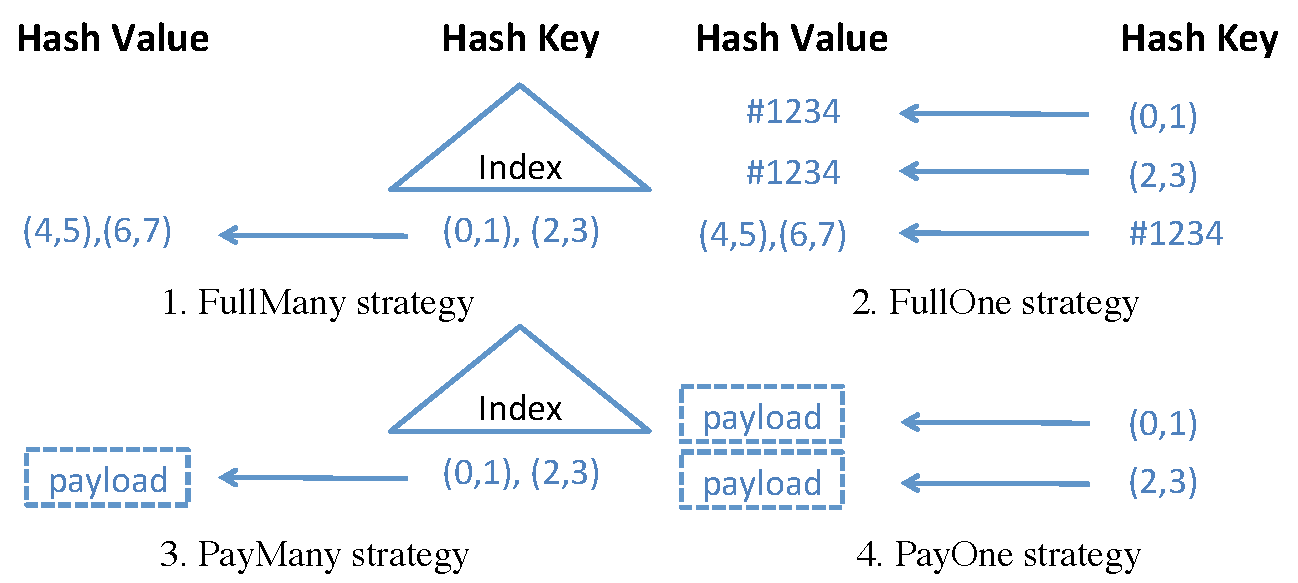
\includegraphics[width=3.1in,natwidth=8.66in,natheight=3.89in]{figures/pointer.pdf}
\caption{ Four examples of encoding strategies }
\label{f:pointer}
\end{center}
\end{figure}

Figure~\ref{f:pointer} depicts how the backward-optimied implementation of
these strategies encode two output cells with coordinates $(0,1)$ and $(2,3)$
that depend on input cells with coordinates $(4,5)$ and $(6,7)$. $FullMany$
uses a single  hash entry with the set of serialized output cells as the key
and the set of input cells as the value (Figure \ref{f:pointer}.1).  Each
coordinate is  bitpacked into a single integer if the array is small enough. We
also create an R\* Tree on the cells in the hash key to quickly find the
entries that intersect with the query. This index uses the dimensions of the
array as its keys and identifies the hash table entries that contain cells in
particular regions.  The figure shows the unserialized versions of the cells
for simplicity.  $FullMany$ is most appropriate when the lineage has high
fanout because it only needs to store the output cells once.

If the fanout is low, $FullOne$ more efficiently serializes and stores each
output cell as the hash key of a separate hash entry.  The hash value stores a reference
to a single entry containing the input cells (Figure \ref{f:pointer}.2).  This implementation doesn't need to
compute and store bounding box information 
and doesn't need the spatial index because each input cell is
stored separately, so queries execute using direct hash lookups.

For payload lineage, $PayMany$ stores the lineage in a similar manner as
$FullMany$, but stores the payload as the hash value
(Figure~\ref{f:pointer}.3).  $PayOne$ creates a hash entry for every output
cell and stores a duplicate of the payload in each hash value
(Figure~\ref{f:pointer}.4).

%In general, $ONE$ is used to
%encode small sets of cells, $MANY$ is used to encode large unique sets of
%cells, while $REF$ is used when a set of cells will be duplicated many times.


%the output cells as a single hash key and creates a spatial index on
%them (Figure \ref{f:pointer}.3), or separately by duplicating the payload for
%each output cell (Figure \ref{f:pointer}.4).  
%Figure \ref{f:pointer} depicts how four of the prevailing backward optimized
%encoding strategies encode a region pair with output cell coordinates $\{(0,1),
%(2,3)\}$ and input coordinates $\{ (4,5),$ $ (6,7) \}$.  
%\noindent {\bf ONE}: Serializes and stores each cell individually
%  by concatenating the  coordinates in each dimension.
%  If the array is small enough, we bitpack the coordinates into a
%  single integer.   \\
%\noindent {\bf MANY}: Serializes and stores the set of cells together.\\
%\noindent {\bf REF}: Stores a reference to the set of cells, which 
%  are encoded using $MANY$ and stored in a separate hash entry.\\
%\noindent {\bf BINARY}: Stores payload as a binary blob.  Reserved for payload lineage.



%We will describe the storage layouts in terms of being optimized for backward lineage
%queries.  We rewrite forward lineage queries, $lwrite(O,
%I_1,\ldots,I_n)$, into $n$ separate calls, $lwrite(I_1, O)$,\ldots,
%$lwrite(I_n, O)$.  We do this because forward queries   \srm{How are those separate calls encoded?   Why do we do
%this? I find this paragraph confusing.}







%$enc_{out}$ can take values of $ONE$, which
%creates a hash entry for each output cell and replicates the serialized input
%cells as the value of each entry, or $MANY$, which stores the output and input
%cells in a single entry, and creates a spatial index on the minimum bounding
%boxes of the output cells.  $enc_{in}$ can take the values of $MANY$, $REF$, or
%$BINARY$. $REF$ stores the cells in a separate hash entry, and keeps a
%reference to the entry with the output cells.  $BINARY$ is dedicated to payload
%data and is stored without modification.




The {\it Optimizer} picks a lineage strategy that spans the entire workflow. It
picks one or more {\it storage strategies} for each operator.  Each storage
strategy is fully specified by a  lineage mode (Full, Map, Payload,
Composite, or Black-box), encoding strategy, and
whether it is forward or backward optimized ($\rightarrow$ or $\leftarrow$).
\sys{} can use multiple storage strategies to optimize for different query types. 


\subsection{Query Execution}
\label{s:qexec}


The {\it Query Executor} iteratively executes each step in the lineage query
path by joining the lineage with the coordinates of the query cells, or the
intermediate cells  generated from the previous step.  The output at each step
is a set of cell coordinates that is compactly stored in an in-memory boolean
array with the same dimensions as the input (backward query) or output (forward
query) array.  A bit is set if the intermediate result contains the
corresponding cell.  For example, suppose we have an operator $P$ that takes as
input a $1\times 4$ array.  Consider a backwards query asking for the lineage
of some output cell $C$ of $P$.  If the result of the query is $1001$, this
means that $C$ depends on the first and fourth cell in $P$'s input.

We chose the in-memory array because many operators have large fanin or fanout,
and can easily generate several times more results (due to duplicates) than are
unique.  De-duplication avoids wasting storage and saves work.  Similarly, the
executor can close an operator early if it detects that all of the possible
cells have been generated.

We also implement an {\it entire array optimization} to speed up queries where
all of the bits in the boolean array are set.  For example, this can happen if
a backward query traverses several high-fanin operators or an all-to-all
operator such as matrix inversion.  In these cases,  calculating the lineage of
every query cell is very expensive and often unnecessary.  Many operators
(e.g., matrix multiply or inverse) can safely assume that the forward
(backward) lineage of an entire input (output) array is the entire output
(input) array.  This optimization is valuable when it can be applied -- it
improved the query performance of a forward query in the astronomy benchmark
that traverses an all-to-all-operator by 83$\times$.

In general, it is difficult to automatically identify when the optimization's
assumptions hold.  Consider a concatenate operator that takes two 2D arrays A,
B with shapes (1, n) and (1, m), and produces an (1, n+m) output by
concatenating B to A.  The optimization would produce different results, because
A's forward lineage is only a subset of the output.  We currently rely on the
programmer to manually annotate operators where the 
optimization can be applied. 



\section{Lineage Strategy Optimizer}
\label{s:optimizer}

Having described the basic storage strategies implemented in \sys{},
we now describe our lineage storage optimizer.
The optimizer's objective is to choose a set of {\it storage strategies} that
minimize the cost of executing the workflow while keeping storage overhead
within user-defined constraints.  We formulate the task as an integer
programming problem, where the inputs are a list of operators, strategy pairs,
disk overheads, query cost estimates, and a sample workload that is used to
derive the frequency with which each operator is invoked in the lineage
workload.  Additionally, users can manually specify operator specific
strategies prior to running the optimizer. 


The formal problem description is stated as:

{\footnotesize
\[
\begin{array}{l l l}
\min_x          & \sum_i p_i * \left(\min_{j|x_{ij}=1} q_{ij}\right) +
&\epsilon * \sum_{ij} (disk_{ij} + \beta * run_{ij}) * x_{ij} \\
%                &\epsilon * \sum_{ij} disk_{ij} * x_{ij} \\
\mbox{s.t.}   &\sum_{ij} disk_{ij} * x_{ij} &\leq MaxDISK\\
              &\sum_{ij} run_{ij} * x_{ij} &\leq MaxRUNTIME\\
              &\forall_{i} \left(\sum_{0 \leq j < M} x_{ij}\right) &\ge 1\\
              &\forall_{i,j} x_{ij} &\in \{0, 1\} \\
&&\\
              &\hspace*{-.3in}  {\rm user\ specified\ strategies}&\\
              &x_{ij} = 1 &\forall_{i,j} x_{ij} \in U
\end{array}
\]
}

Here, $x_{ij} = 1$ if operator $i$ stores lineage using strategy $j$, and 0
otherwise.  $MaxDISK$ is the maximum storage overhead specified by the user;
$q_{ij}$, $run_{ij}$, and $disk_{ij}$, are the average query cost, runtime
overhead, and storage overhead costs for operator $i$ using strategy $j$ as
computed by the cost model.  $p_{ij}$ is the probability that a lineage
query in the workload accesses operator $i$, and is computed from the sample
workload.  A single operator may store its lineage data using multiple
strategies.

The goal of the objective function is to minimize the cost of executing the
lineage workload, preferring strategies that use less storage.  When an
operator uses multiple strategies to store its lineage, the query processor
picks the strategy that minimizes the query cost.  The $\min$ statement in the
left hand term picks the best query performance from the strategies that have
been picked ($j | x_{ij} = 1$).  The right hand term penalizes strategies that
take excessive disk space or cause runtime slowdown.  $\beta$ weights runtime
against disk overhead, and $\epsilon$ is set to a very small value to break
ties. A large $\epsilon$ is similar to reducing $MaxDISK$ or $MaxRUNTIME$.

We heuristically remove configurations that are clearly non-optimal, such as
strategies that exceed user constraints, or are not properly indexed for any of
the queries in the workload (e.g., forward optimized when the workload only
contains backward queries).  The optimizer also picks mapping functions over
all other classes of lineage.

We solve the ILP problem using the simplex method in GNU Linear Programming
Kit.  The solver takes about 1ms to solve the problem for the 
benchmarks.




\subsection{Query-time Optimizer}
\label{s:cmopt}

While the lineage strategy optimizer picks the optimal lineage strategy, the
executor must still pick between accessing the lineage stored by one of the
lineage strategies, or re-running the operator.  The query-time optimizer
consults the cost model using statistics gathered during query execution and
the size of the query result so far to pick the best execution method.  In
addition, the optimizer monitors the time to access the materialized lineage.
If it exceeds the cost of re-executing the operator, \sys{} dynamically
switches to re-running the operator.  This bounds the worst case performance to
2$\times$ the black-box approach.







\section{Experiments}
\label{s:expt}




\begin{table}[tb]
\begin{center}
\footnotesize
\caption{Lineage Strategies for experiments.}
  \begin{tabular}{ | l | l | }
    \hline
    {\bf Strategy} &  {\bf Description} \\ \hline \hline
    \multicolumn{2}{|c|}{\bf Astronomy Benchmark} \\ \hline
    BlackBox & All operators store black-box lineage \\ \hline
    BlackBoxOpt & Like BlackBox, uses mapping lineage for built-in-operators.\\ \hline
    FullOne & Like BlackBoxOpt, but uses FullOne for UDFs.\\ \hline
    FullMany & Like FullOne, but uses FullMany for UDFs.\\ \hline
    Subzero & Like FullOne, but stores composite lineage\\
            & using PayOne for UDFs.\\ \hline
    \multicolumn{2}{|c|}{\bf Genomics Benchmark} \\ \hline
    BlackBox & UDFs store black-box lineage \\ \hline
    FullOne & UDFs store backward optimized FullOne\\ \hline
    FullMany & UDFs store backward optimized FullMany\\ \hline
    FullForw & UDFs store forward optimized FullOne\\ \hline
    FullBoth & UDFs store FullForw and FullOne \\ \hline
    PayOne & UDFs store PayOne\\ \hline
    PayMany & UDFs store PayMany\\ \hline
    PayBoth & UDFs store PayOne and FullForw\\ \hline
\end{tabular}
\end{center}
\label{t:strats}
\end{table}

In the following subsections, we first describe how \sys{} optimizes the
storage strategies for the real-world benchmarks described in
Section~\ref{s:usecases}, then compare several of  our lineage storage
techniques with black-box level only techniques.  The astronomy benchmark shows
how our region lineage techniques improve over cell-level and black-box
strategies on  an image processing workflow.   The genomics benchmark
illustrates the complexity in determining an optimal lineage strategy and that
the the optimizer is able to  choose an effective strategy within user
constraints.


Overall, our findings are that:
\begin{itemize}

\item An optimal strategy heavily relies on operator properties such as fanin,
    and fanout, the specific lineage queries, and query execution-time
    optimizations.  The difference between a sub-optimal and optimal strategy
    can be so large that an optimizer-based approach is crucial.

\item Payload, composite, and mapping lineage are extremely effective and
    low overhead techniques that greatly improve query performance, and are
    applicable across a number of scientific domains.

\item  \sys{} can improve the LSST benchmark queries by up to 10$\times$
    compared to naively storing the region lineage (similar to what
    cell-level approaches would do) and up to 255$\times$ faster than black-box
    lineage.   The runtime and storage overhead of the optimal scheme is up to
    30 and 70$\times$ lower than cell-level lineage, respectively, and only
    1.49 and 1.95$\times$ higher than executing the workflow.

\item Even though the genomics benchmark executes operators very quickly,
    \sys{} can find the optimal mix of black-box and region lineage that scales
    to the amount of available storage.  \sys{} uses a black-box only strategy
    when the available storage is small, and switches from space-efficient to
    query-optimized encodings with looser constraints.  When the storage
    constraints are unbounded, \sys{} improves forward queries by over
    500$\times$ and backward queries by 2-3$\times$.

\end{itemize}

The current prototype is written in Python and uses BerkeleyDB for the
persistent store, and libspatialindex for the spatial index.  The
microbenchmarks are run on a 2.3 GHz linux server with 24 GB of RAM, running
Ubuntu 2.6.38-13-server.  The benchmarks are run on a 2.3 GHz MacBook Pro with
8 GB of RAM, a 5400 RPM hard disk, running OS X 10.7.2.

\subsection{Astronomy Benchmark}





\begin{figure}[htb]
\advance\leftskip-.1in
\subfigure[Disk and runtime overhead]
{
    \label{f:overhead1}
     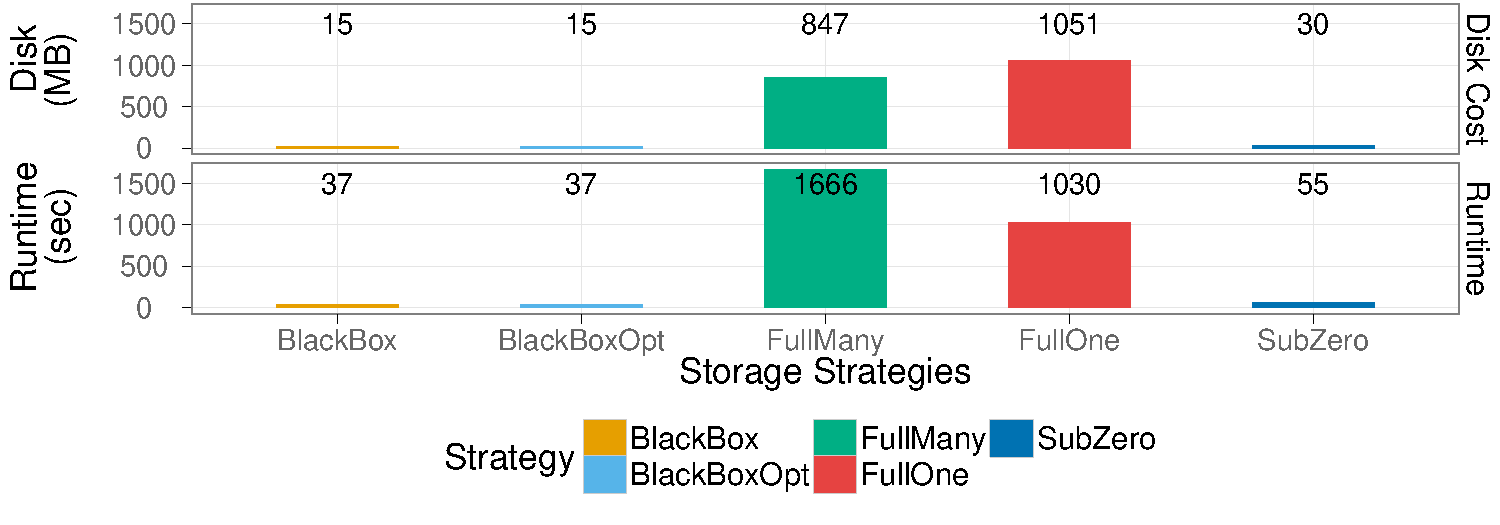
\includegraphics[width=3.5in,natwidth=10in,natheight=3.5in]{figures/lsst/overhead.pdf}
}
\subfigure[Query costs. Y-axes are log scale]
{
    \label{f:cost1}
    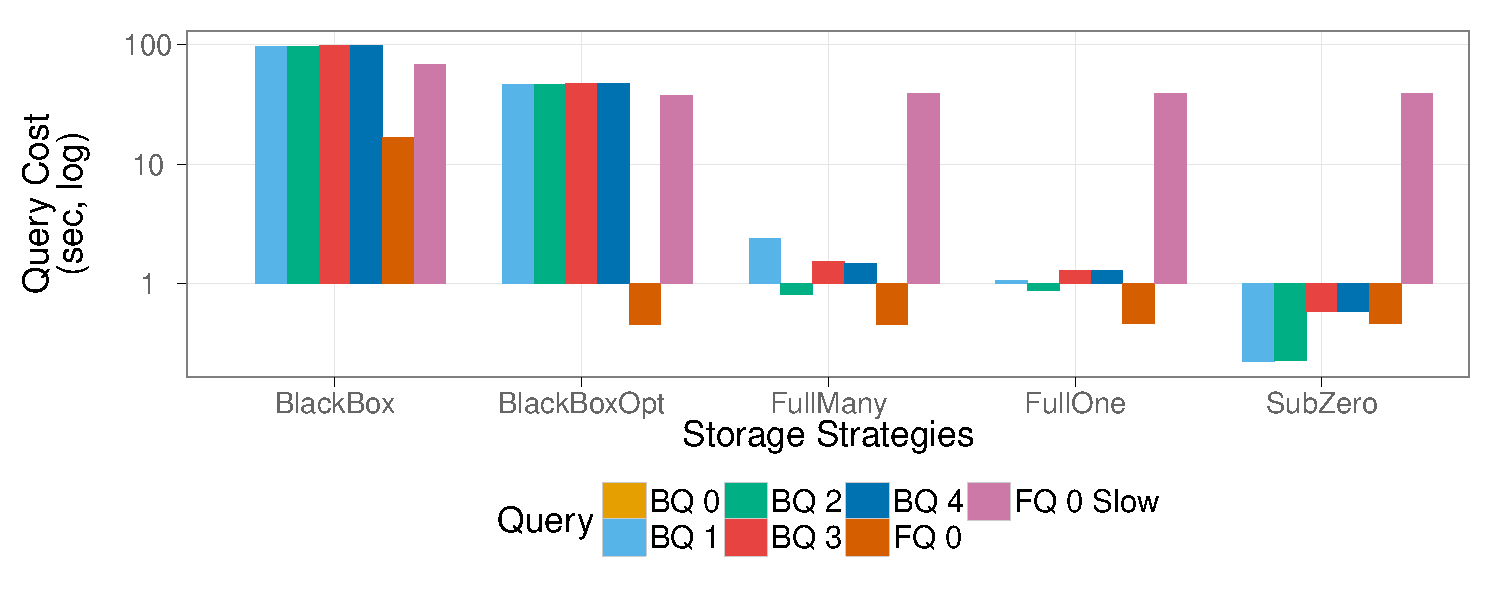
\includegraphics[width=3.5in,natwidth=10in,natheight=4in]{figures/lsst/cost.pdf}
}
\advance\rightskip-.2in
\caption{Astronomy Benchmark}
\label{f:lsst}
\end{figure}


In this experiment, we run the Astronomy workflow with  five backward
queries and one forward query as described in Section \ref{s:ucastro}.  The 22
built-in operators are all expressed as mapping operators and the UDFs consist
of one payload operator that detects celestial bodies and three composite
operators that detect and remove cosmic rays.  This workflow exhibits
considerable locality (stars only depend on neighboring pixels), sparsity
(stars are rare and small), and the queries are primarily backward queries.
Each workflow execution consumes two 512$\times$2000 pixel (8MB) images
(provided by LSST) as input, and we compare the strategies in Table \ref{t:strats}.

Figure \ref{f:overhead1} plots the disk and runtime overhead for each of the
strategies. $BlackBox$ and $BlackBoxOpt$ show the base cost to execute the
workflow and the size of the input arrays -- the goal is to be as close to
these bars as possible.  $FullOne$ and $FullMany$ both require considerable
storage space (66$\times$, 53$\times$) because the three cosmic ray operators
generate a region pair for every input and output pixel at the same
coordinates.  Similarly, both approaches incur 6$\times$ and 44$\times$ runtime
overhead to serialize and store them.  $FullMany$ must also
construct the spatial index on the output cells.  The \sys{} optimizer instead
picks composite lineage that only stores payload lineage for the small
number of cosmic rays and stars.  This reduces the runtime and disk overheads
to 1.49$\times$ and 1.95$\times$ the workflow inputs.  By comparison, this
storage overhead is negligible compared to the cost of storing the intermediate
and final results (which amount to 11.5$\times$ the input size).


Figure \ref{f:cost1} compares lineage query execution costs. $BQ~x$ and $FQ~x$
respectively stand for backward and forward query x.  All of the queries use
the entire array optimization described in Section \ref{s:qexec} whereas $FQ 0
Slow$ does not.  $BlackBox$ must re-run each operator and takes up to 100 secs
per query.  $BlackBoxOpt$ can avoid rerunning the mapping operators, but still
re-runs the computationally intensive UDFs.  Storing region lineage reduces
the cost of executing the backward queries by 34$\times$ ($FullMany$) and
$45\times$ ($FullOne$) on average.  \sys{} benefits from executing mapping
functions and reading a small amount of lineage data and executes 255$\times$
faster on average.  $FQ\ 0\ Slow$ illustrates how the all-to-all optimization
improves the query performance by 83$\times$ by avoiding fine-grained lineage
all-together.
















\subsection{Genomics Benchmark}




\begin{figure}[t]
\vspace{-.1in}
\advance\leftskip-.05in
\subfigure[Disk and runtime overhead]
{
    \label{f:goverhead}
    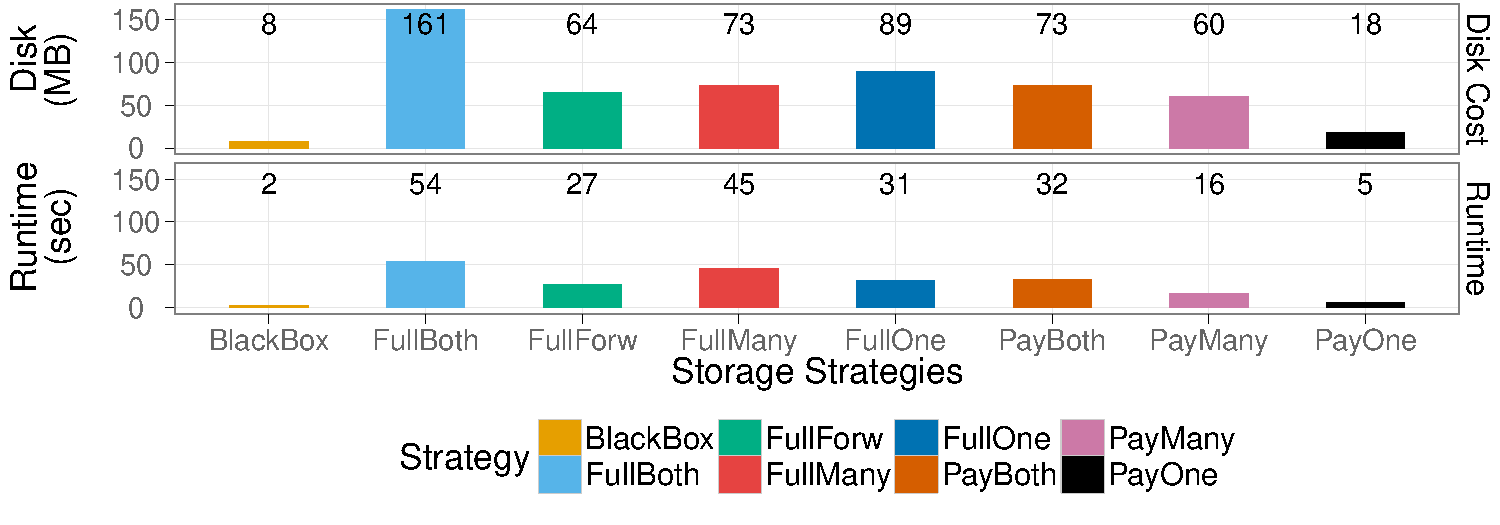
\includegraphics[width=3.5in,natwidth=10in,natheight=3.5in]{figures/genomics/overhead_noopt.pdf}
}
\subfigure[Query costs (static).  Y-axes are log scale.]
{
    \label{f:gcosts100_static}
     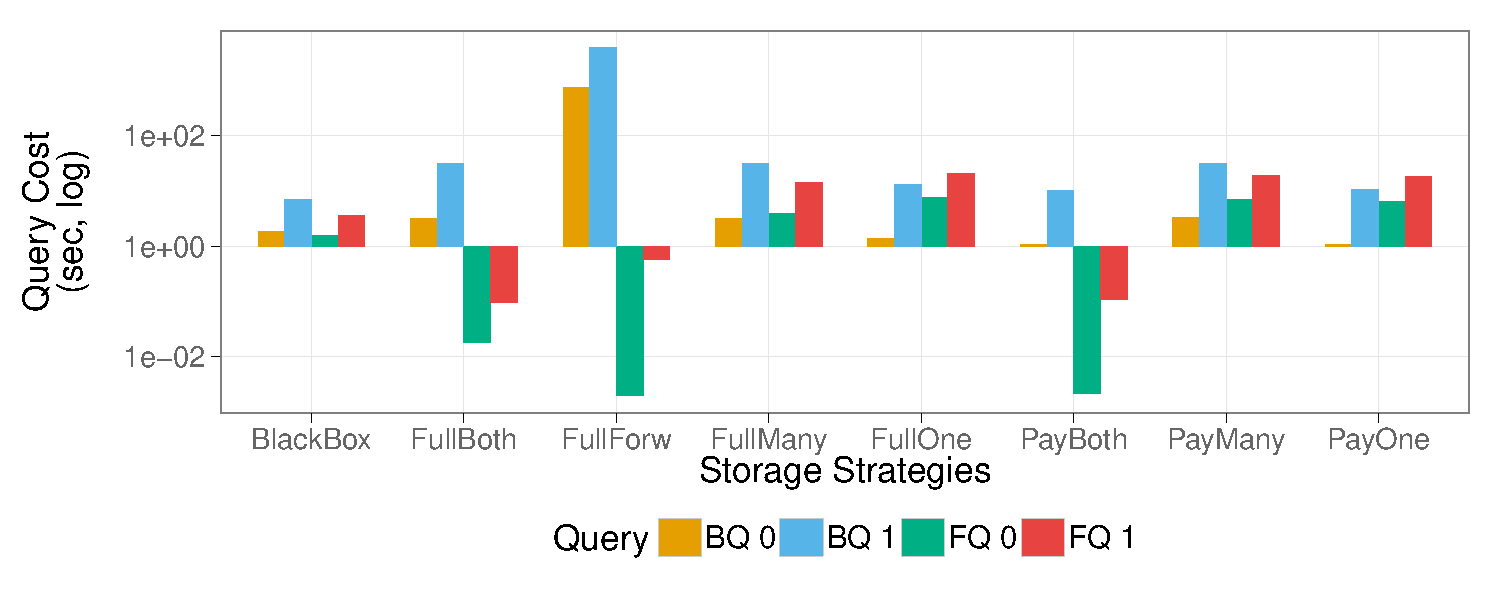
\includegraphics[width=3.5in,natwidth=10in,natheight=4in]{figures/genomics/cost_static.pdf}
}
\subfigure[Query costs (dynamic). Y-axes are log scale.]
{
    \label{f:gcosts100_dynamic}
     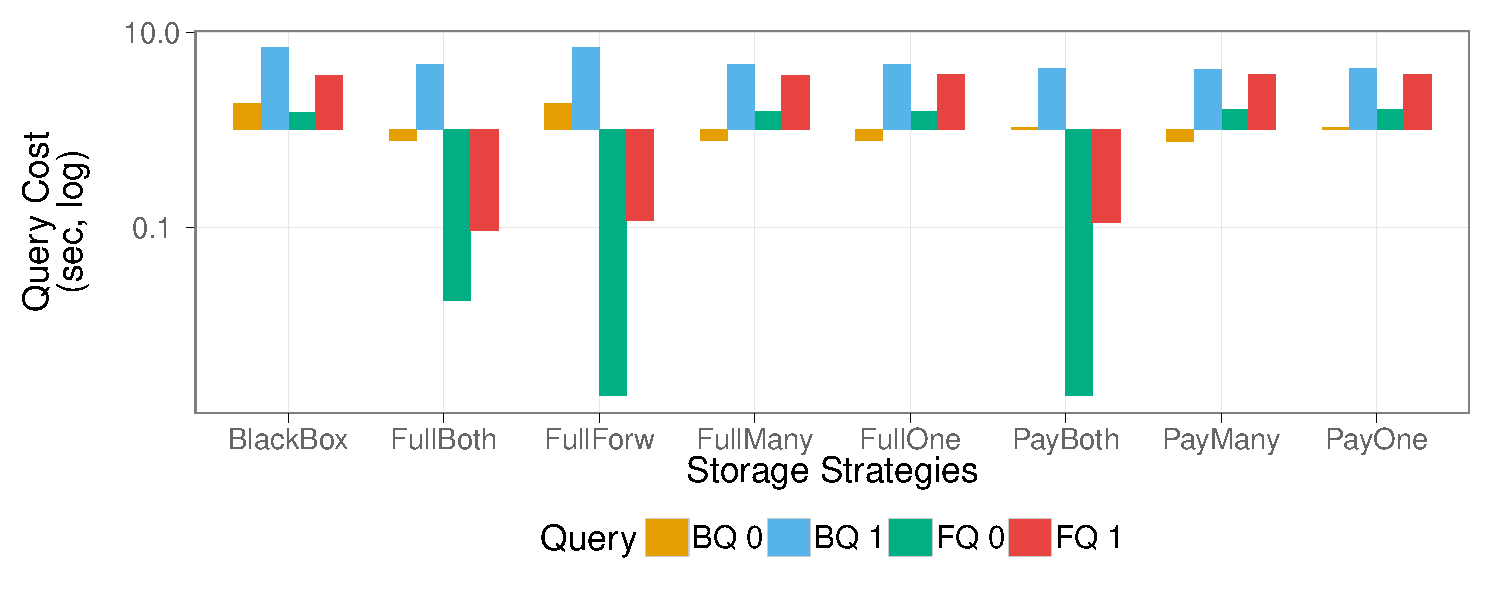
\includegraphics[width=3.5in,natwidth=10in,natheight=4in]{figures/genomics/cost_dynamic.pdf}
}
\advance\rightskip-.2in
\caption{Genomics benchmark.  Queries run
  with (dynamic) and without (static) the query-time optimizer
  described in Section \ref{s:cmopt}.}
\label{f:genomics1}
\end{figure}

In this experiment, we run the genomics workflow and execute a
lineage workload with an equal mix of forward and backward
lineage queries (Section \ref{s:ucgenomics}).  There are 10
built-in mapping operators, and the 4 UDFs are all payload operators.
In contrast to the astronomy workflow, these UDFs do not exhibit
significant locality, and perform data shuffling and extraction
operations that are not amenable to mapping functions.  In addition,
the operators perform simple calculations, and execute quickly, so
there is a less pronounced trade off between re-executing the workflow
and accessing region lineage.  In fact, there are cases where
storing lineage actually {\it degrades} the query performance.  We
were provided a 56$\times$100 matrix of 96 patients and 55 health and
genetic features.  Although the dataset is small, future datasets are
expected to come from a larger group of patients, so we constructed
larger datasets by replicating the patient data. The
query performance and overheads scaled linearly with the size of the
dataset and so we report results for the dataset scaled by 100$\times$.

We first show the high variability between different static strategies (Table
\ref{t:strats}) and how the query-time optimizer (Section~\ref{s:cmopt})
avoids sub-optimal query execution.  We then show how the \sys{} cost based
optimizer can identify the optimal strategy within varying user constraints.



\subsubsection{Query-Time Optimizer}
\label{s:genomicsfixed}

This experiment compares the strategies in Table~\ref{t:strats} with and
without the query-time optimization described in Section~\ref{s:cmopt}.  Each
operator uses mapping lineage if possible, and otherwise stores lineage
using the specified strategy.  The majority of the UDFs generate region pairs
that contain a single output cell.  As mentioned in previous experiments,
payload lineage stores very little binary data, and incurs less overhead
than the full lineage approaches (Figure~\ref{f:goverhead}).  Storing both
forward and backward-optimized lineage ($PayBoth$ and $FullBoth$) requires
significantly more overhead --  8 and 18.5$\times$ more space than the input
arrays, and 2.8 and 26$\times$ runtime slowdown.

Figure \ref{f:gcosts100_static} highlights how query performance can {\it
degrade} if the executor blindly joins queries with mismatched indexed lineage
(e.g., backward-optimized lineage with forward queries)\footnote{ All
comparisons are relative to $BlackBox$}.  For example, $FullForw$ degraded
backward query performance by 520$\times$.  Interestingly, the BQ1 ran slower
because the query path contains several operators with very large fanins.  This
generates so many intermediate results that performing index lookups on each
one is slower than re-running the operators.  Note however, that the forward
optimized strategies improved the performance of FQ0 and FQ2 because the fanout
is low.

Figure~\ref{f:gcosts100_dynamic} shows that the query-time optimizer executes
the queries as fast as, or faster than, $BlackBox$. In general, this
requires accurate statistics and cost estimation, the optimizer limits the
query performance degradation to 2$\times$ by dynamically switching to the
$BlackBox$ strategy.  Overall, the backward and forward queries improved by up
to 2 and 25$\times$, respectively.








\subsubsection{Lineage Strategy Optimizer}

\begin{figure}[tb]
\vspace{-.1in}
\advance\leftskip-.05in
\subfigure[Disk and runtime overhead]
{
    \label{f:goverhead_opt}
     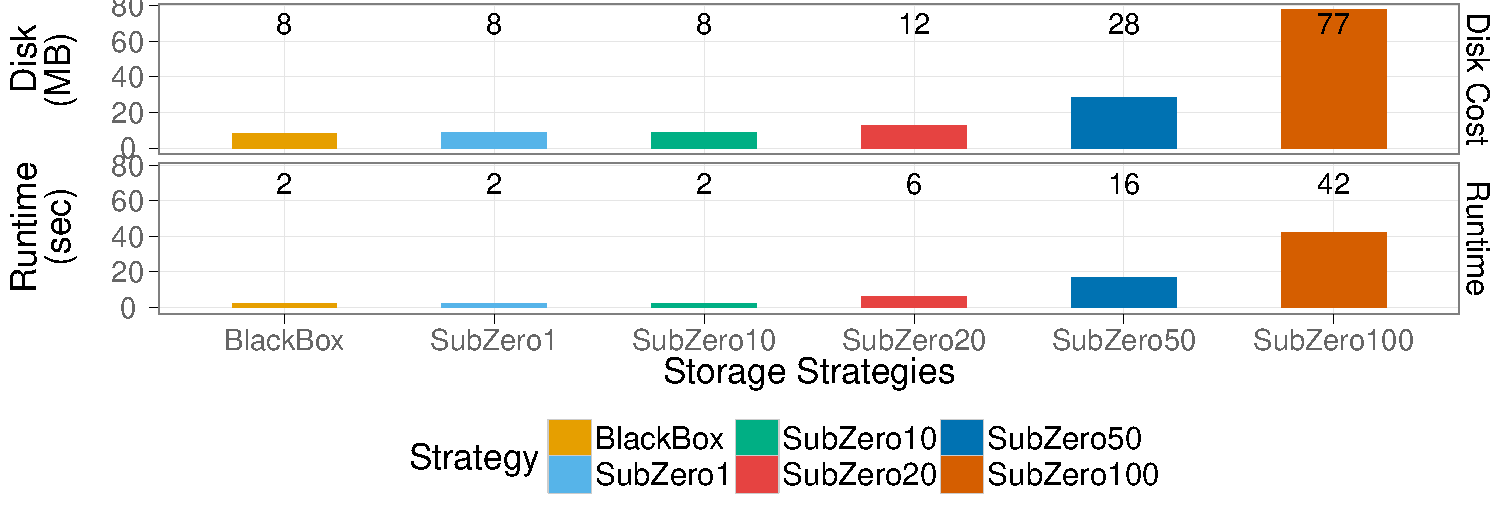
\includegraphics[width=3.5in,natwidth=10in,natheight=3.5in]{figures/genomics/overhead_opt.pdf}
}
\subfigure[Query costs.  Y-axes are log scale.]
{
    \label{f:gcosts100_opt}
     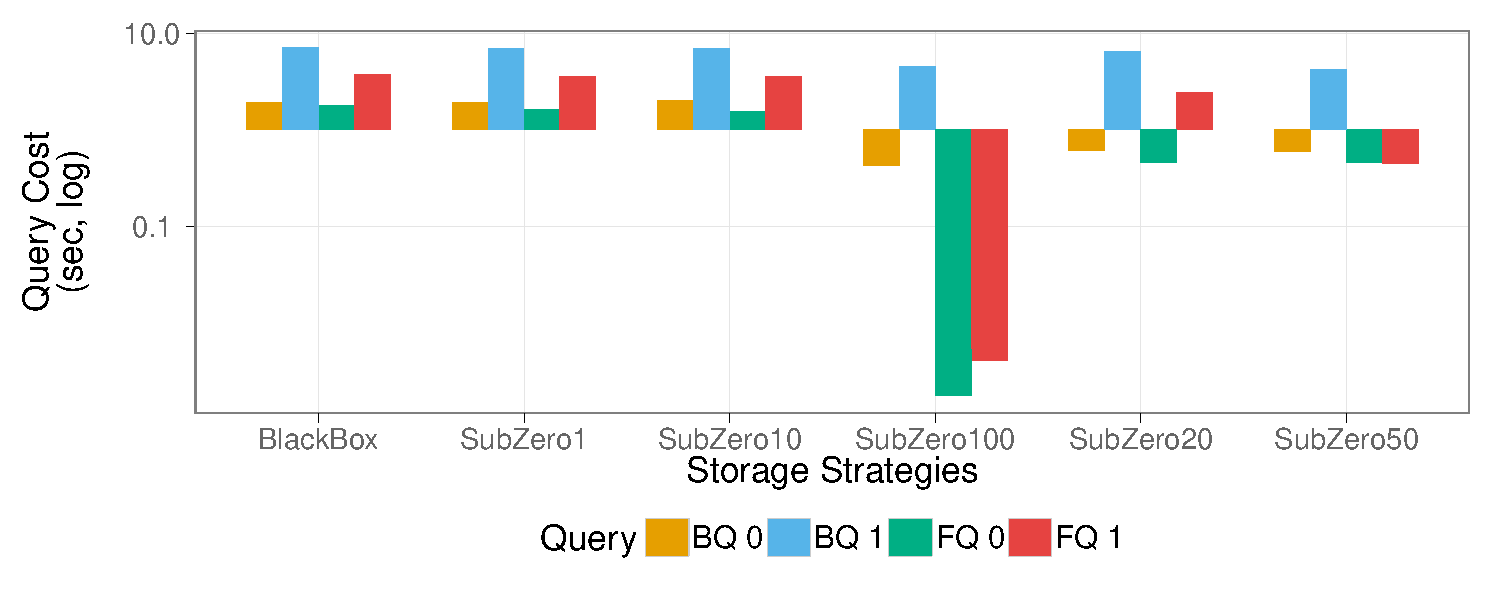
\includegraphics[width=3.5in,natwidth=10in,natheight=4in]{figures/genomics/cost_opt.pdf}
}
\advance\rightskip-.2in
\caption{Genomics benchmark.  SubZero{\it X} has storage constraint {\it X} MB }
\vspace{.1in}
\label{f:goptimizer}
\end{figure}



The previous section compared many strategies, each with different performance
characteristics depending on the operator and query.  We now evaluate the
\sys{} strategy optimizer on the genomics benchmark. Figure \ref{f:goptimizer}
illustrates that when the user increases storage constraints from 1 to 100MB
(with unbounded runtime constraint), the optimizer picks more storage intensive
strategies that are predicted to improve the benchmark queries.  \sys{} chooses
$BlackBox$ when the constraint is too small, and stores forward and
backward-optimized lineage that benefits all of the queries when the minimum
amount of storage is available (20MB).  Materializing further lineage has
diminishing storage-to-query benefits.  $SubZero100$ uses 50MB to
forward-optimize the UDFs using $(MANY, ONE)$, which reduces the forward query
costs to sub-second costs. This is because the UDFs have low fanout, so each
join in the query path is a small number of hash lookups.  Due to space
constraints, we simply mention that specifying and varying the runtime overhead
constraints achieves similar results.




\subsection{Microbenchmark}


The previous experiments compared several end-to-end strategies, however it can
be difficult to distinguish  the sources of the benefits.  This
subsections summarizes the key differences between the prevailing strategies in
terms of overhead and query performance.  The comparisons use an operator that
generates synthetic lineage data with tunable parameters.  Due to space
constraints we show results from varying the fanin, fanout and payload size
(for payload lineage).


%for the lineage
%fanin and fanout ($fanin$ \& $fanout$), the payload size for payload lineage,
%and the number of output cells containing lineage that are generated
%($noutput$).  Due to space constraints we report results where $noutput=10\%$
%of the output array.  The results scale close to linearly with $noutput$.

Each experiment processes and outputs a 1000x1000 array, and generates lineage
for 10\% of the output cells.  The results scaled close to linearly as the
number of output cells with lineage varies.   A region pair is
randomly generated by  selecting a cluster of output cells with a radius
defined by $fanout$, and selecting $fanin$  cells in the same area from the
input array.   We generate region pairs until the total number of output cells
is equal to 10\% of the output array.  The payload strategy uses a payload size
of {\it fanin}$\times${\it 4 bytes} (the payload is expected to be very small).
We compare several backward optimized strategies ($\leftarrow FullMany$,
$\leftarrow FullOne$, $\leftarrow PayMany$, $\leftarrow PayOne$), one forward
lineage strategy ($\rightarrow FullOne$), and black-box ($BlackBox$).   We
first discuss the overhead to store and index the lineage, then comment on
the query costs.


Figure \ref{f:micro_overhead} compares the runtime and disk overhead of the
different strategies.  For referenc, the size of the input array is 3.8MB.  The
best full lineage strategy differs based on the operator fanout. $FullOne$ is
superior when $fanout \le 5$ because it doesn't need to create and store the
spatial index.  The crossover point to $FullMany$ occurs when the cost of
duplicating hash entries for each output cell in a region pair exceeds that of
the spatial index.  The overhead of both approaches increases with fanin.  In
contrast, payload lineage has a much lower overhead than the full lineage
approaches and is independent of the fanin because the payload is typically
small and does not need to be encoded.  When the fanout increases to 50 or 100,
$PayMany$ and $FullMany$ require less than 3MB and 1 second of overhead.
 The forward optimized $FullOne$ is comparable to
the other approaches when the fanin is low.   However, when the fanin increases
it can require up to $fanin\times$ more hash entries because it creates an
entry for every distinct input cell in the lineage.  It converges to the
backward optimized $FullOne$ when the fanout and fanin are high. Finally,
$BlackBox$ has nearly no overhead.

Figure \ref{f:micro_query} shows that the query performance for queries that
access the backward/forward lineage of 1000 output/input cells.  The
performance scales mostly linearly with the query size.  There is a clear
difference between $FullMany$ or $PayMany$, and $FullOne$ or $PayOne$, due to
the additional cost of accessing the spatial index (Figure
\ref{f:micro_query}).  Payload lineage performs similar to, but not
significantly faster than full provenance, although the query performance
remains constant as the fanin increases.    In comparison (not shown),
$BlackBox$ takes between 2 to 20 seconds to execute a query where {\it fanin=1}
and around 0.7 seconds when {\it fanin=100}.  Using a mis-matched index (e.g,
using forward-optimized lineage for backward queries) takes up to two orders of
magnitude longer than $BlackBox$ to execute the same queries.  The forward
queries using $\rightarrow FullOne$ execute similarly to $\leftarrow FullOne$
in Figure~\ref{f:micro_query} so we do not include the plots.
%\srm{Figure  \ref{f:micro_query}(b) is pretty boring, since you aren't
%comparing anything!}

%\begin{figure}[ht]
%\advance\leftskip-.3in
%\subfigure[Disk Overhead]
%{
%    \label{f:micro_disk}
%    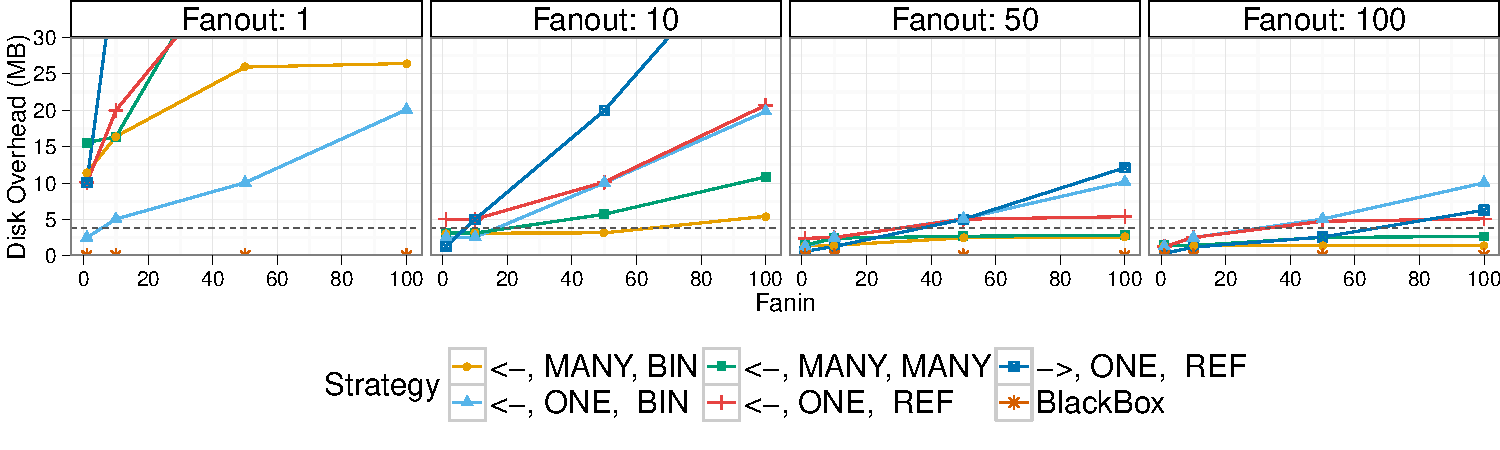
\includegraphics[width=3.7in]{figures/microbench/disk}
%}\\
%\subfigure[Runtime Overhead]
%{
%    \label{f:micro_runtime}
%    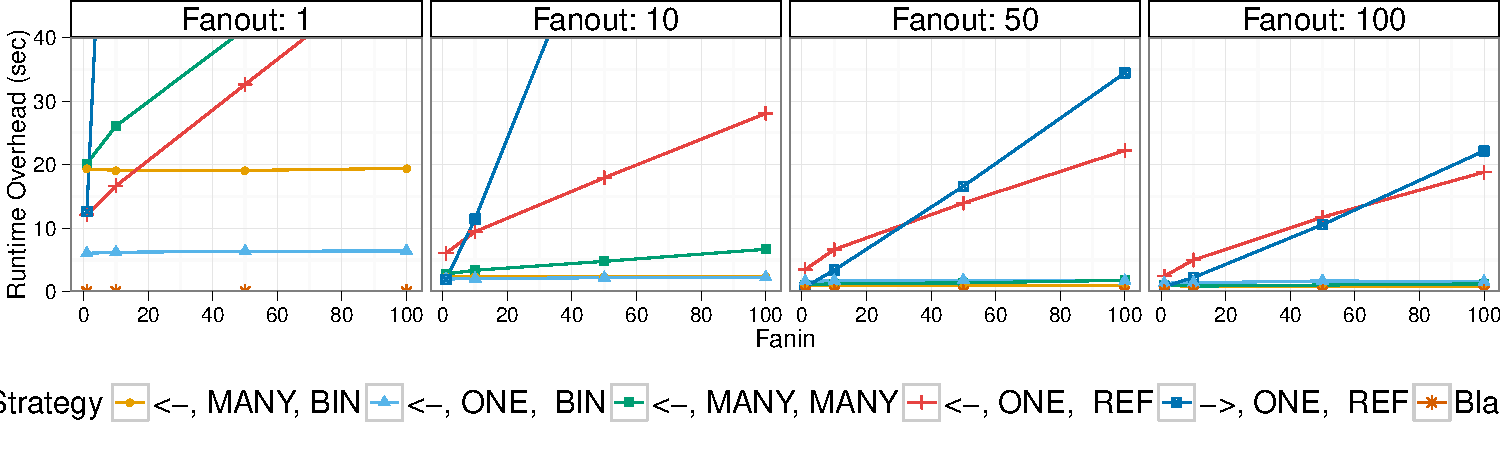
\includegraphics[width=3.7in]{figures/microbench/runtime}
%}
%%\advance\rightskip-.2in
%\vspace{-.2in}
%\caption{Disk and runtime overhead}
%\label{f:micro_overhead}
%\end{figure}


\begin{figure}[ht]
%\advance\leftskip-.2in
    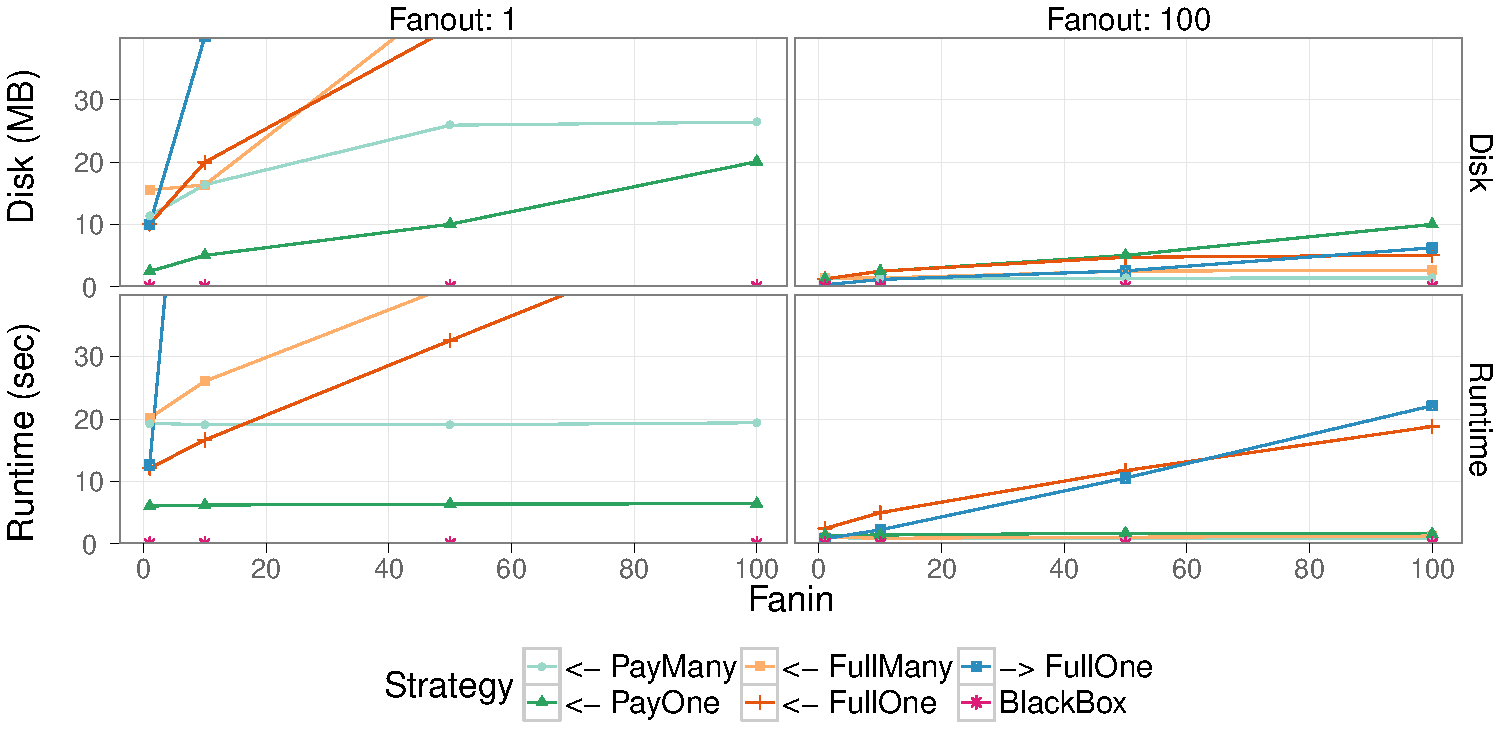
\includegraphics[width=3.7in,natwidth=10in,natheight=5in]{figures/microbench/overhead.pdf}
%\advance\rightskip-.2in
\vspace{-.2in}
\caption{Disk and runtime overhead}
\label{f:micro_overhead}
\end{figure}

\begin{figure}[htb]
%\advance\leftskip-.3in
    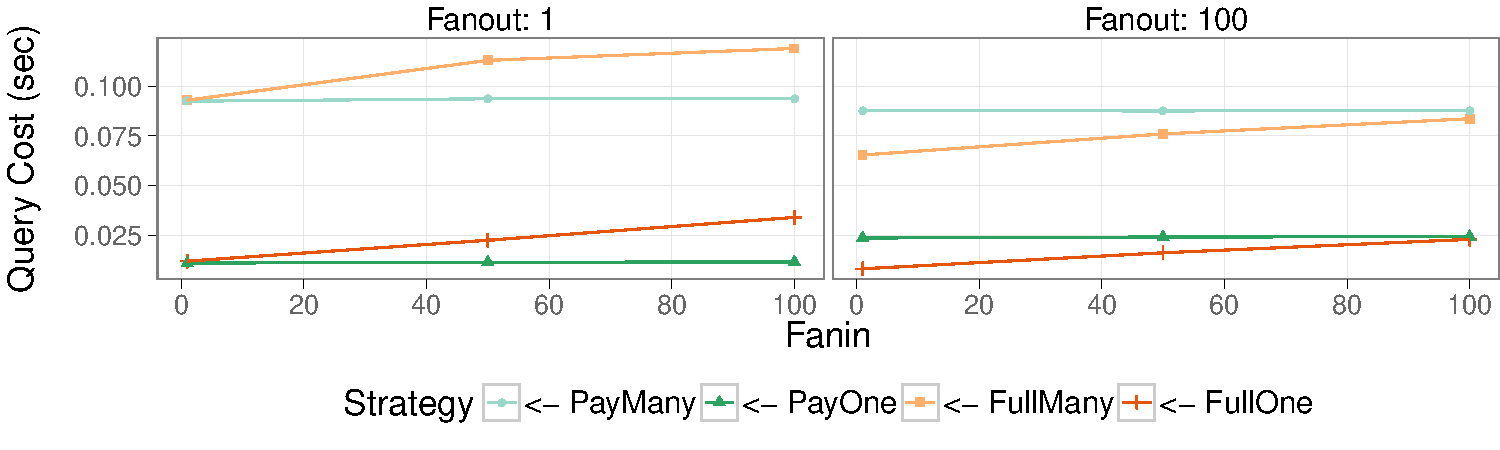
\includegraphics[width=3.6in,natwidth=10in,natheight=3in]{figures/microbench/query_back.pdf}
%\advance\rightskip-.2in
%\vspace{-.2in}
\caption{Backward Lineage Queries, only backward-optimized strategies}
\label{f:micro_query}
\end{figure}




%\begin{figure}[htb]
%%\advance\leftskip-.3in
%\subfigure[Backward Queries, only backward-optimized strategies]
%{
%    \label{f:micro_bq}
%    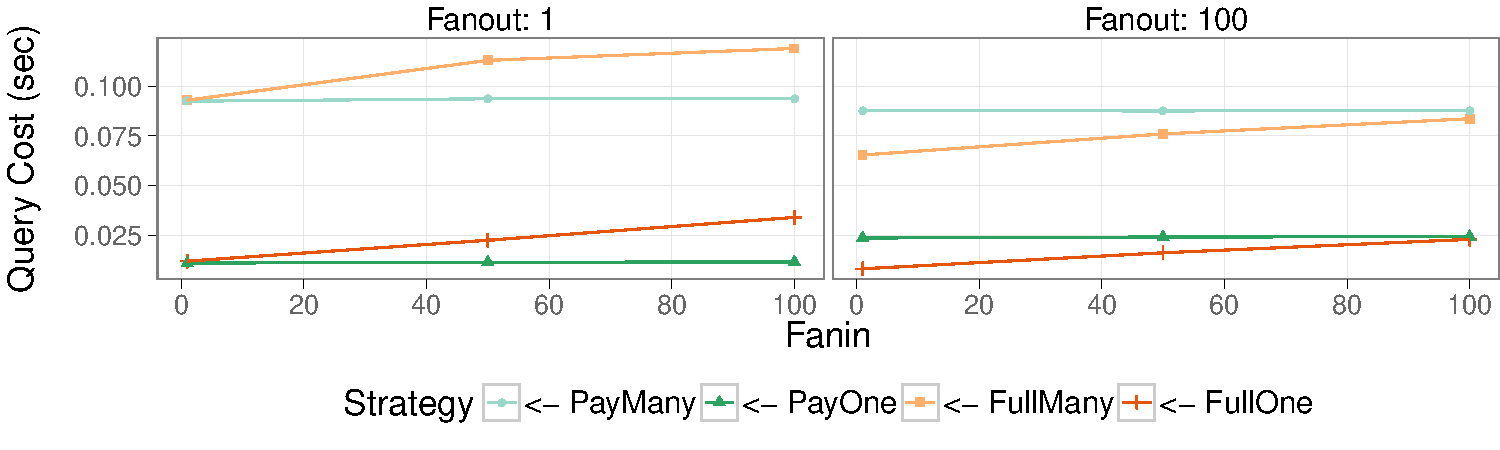
\includegraphics[width=3.6in]{figures/microbench/query_back}
%}\\
%\subfigure[Forward Queries, only forward-optimized strategies]
%{
%    \label{f:micro_fq}
%    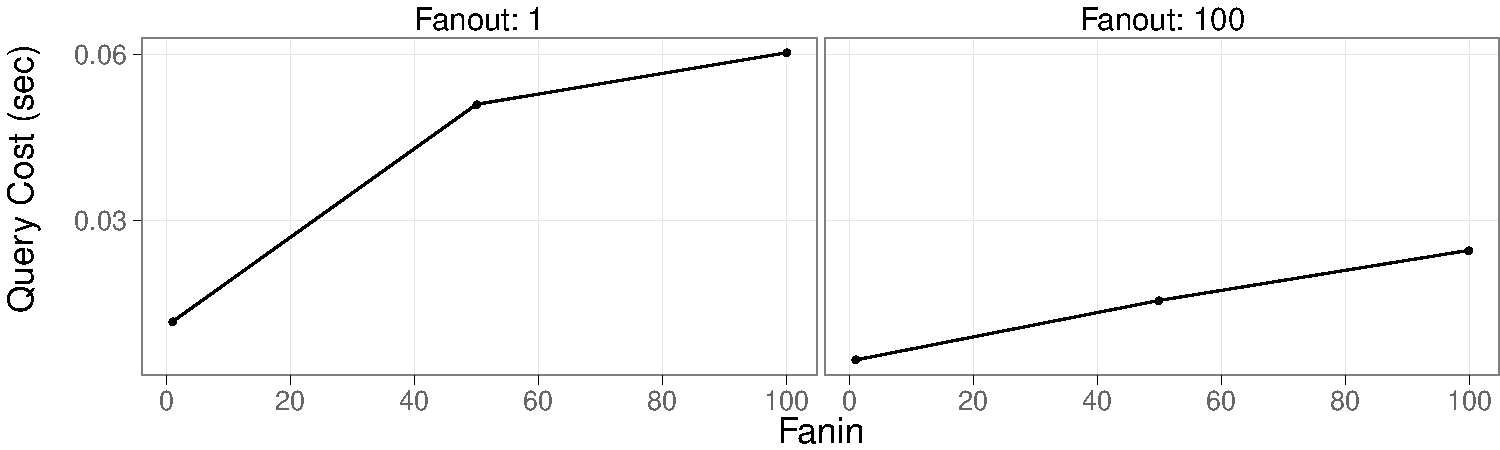
\includegraphics[width=3.6in]{figures/microbench/query_forw}
%}
%%\advance\rightskip-.2in
%%\vspace{-.2in}
%\caption{Backward and Forward lineage query costs.}
%\label{f:micro_query}
%\end{figure}



%The storage strategy is tied to the lineage queries and user preferences
%between workflow execution overhead and lineage query performance.  Poorly
%designed systems can easily incur three orders of magnitude of runtime
%overhead, 4$\times$ the disk overhead, and two orders of magnitude query slow
%down.




\subsection{Discussion}

The experiments show that the best strategy is tied to the
operator's lineage properties, and that there are orders of magnitude
differences between different lineage strategies.   Science-oriented lineage
systems should seek to identify and exploit operator fanin, fanout, and
redundancy properties.

Many scientific applications -- particularly sensor-based or image processing
applications like environmental monitoring or astronomy -- exhibit substantial
locality (e.g., average temperature readings within an area) that can be used
to define payload, mapping or composite operators.  As the experiments show,
\sys{} can  record their lineage with less overhead than from operators that
only support full lineage. When locality is not present, as in the genomics
benchmark,  the optimizer may still be able to find opportunities to record
lineage if the constraints are relaxed.  A very promising alternative is to
simplify the process of writing payload and mapping functions by supporting
variable granularities of lineage.  This lets developers define coarser
relationships between input and outputs (e.g., specify lineage as a bounding
box that may contain inputs that didn't contribute to the output). This also
allows the lineage system perform lossy compression.

%The experiments showed that the slowdown caused by  storing lineage
%can dwarf the cost of executing the application (e.g., the genomics benchmark),
%which is unacceptable in scenarios such as real-time applications.  In these
%cases, the optimizer will choose black-box lineage.  However, as evidenced in
%the genomics benchmark and the microbenchmarks, \sys{} can still improve query
%peformance by efficiently store lineage for high fanout operators or operators
%that support payload lineage.

%Although our region provenance encodings are applicable to a large class of
%scientific operators, if may be difficult to define  mapping functions or  the
%correct $lwrite$ calls for complex UDFs.  In these cases, the developer may opt
%to adopt a coarser definition of lineage by specifying coarse regions of input
%cells. While out of the scope of this paper, supporting and optimizing varying
%granularities of lineage is a promising future direction.


%Finally, there may be times where the lineage is very expensive to store but is
%not  {\it useful} (e.g., kmeans just references everything), and sometimes the
%lineage is very large, which motivates the DBWipes stuff we are doing. Maybe we
%should just reference what we're doing as ``future work?''}


%
%The microbenchmarks showed that the runtime overhead increases as more
%lineage is stored. For example, the runtime overhead was up to 50$\times$ in
%the genomics benchmark. This may be unacceptable for applications with
%real-time requirements (forcing our optimizer to choose to just use black box
%lineage).  However, even strict constraints can provide benefits -- the
%$PayOne$ strategy in Figure~\ref{f:genomics1}(c) reduced backwards query costs
%by about 50\% while imposing a very small runtime penalty.  Other applications,
%such as the genomic visualization that interactively executes lineage
%queries, may be willing to incur offline overhead in order to minimize query
%runtimes.

%We also note that many scientific applications -- particularly sensor-based or
%image processing applications like environmental monitoring or astronomy --
%exhibit substantial locality (e.g., average temperature readings within an
%area) that can be used to define payload, mapping or composite operators.


%\red{Highlight how powerful composite lineage is.  Talk about
%    programmability -- many readers will worry that some operators are simply
%    very difficult write $lwrite$ functions for.  I actually think that many
%    UDFs may be very complicated, but the input to output relationships should
%    ultimately be pretty obvious (perhaps at a coarser grain).  Often


\section{Related Work}


%Many of our ideas are
%inspired by previous work, which we highlight in this section.


There is a long history of provenance and lineage research both in database
systems and in more general workflow systems.   There are several excellent
surveys that characterize provenance in databases~\cite{provdb} and scientific
workflows~\cite{provsci,provsci2}.  As noted in the introduction, the primary
differences from prior work  are that \sys{} uses a mix of black-box and region
provenance, exploits the semantics of scientific operators (making using of
mapping functions) and uses a number of provenance encodings.  

Most workflow systems support custom operators containing user-designed code
that is opaque to the runtime.  This presents a difficulty when trying to
manage cell-level (e.g., array cells or database tuples) provenance.  Some
systems~\cite{genepattern,galaxy} model operators as black-boxes where all
outputs depend on all inputs, and track the dependencies between input and
output datasets.  Efficient methods to expose, store and query cell-level
provenance is an area of on-going research.

Several projects exploit workflow systems that use high level programming
constructs with well defined semantics.  RAMP~\cite{ramp} extends MapReduce to
automatically generate lineage capturing wrappers around Map and Reduce
operators.  Similarly, Amsterdamer et al~\cite{lipstick} instrument the
PIG~\cite{pig} framework to track the lineage of PIG operators.  However,
 user defined operators are treated as black-boxes, which limits their ability to
track lineage. 

Other workflow systems (e.g., Taverna~\cite{taverna} and Kepler~\cite{kepler}),
process nested collections of data, where  data items may be  imagees or DNA
sequences.  Operators  process  data items in a collection, and these systems
automatically track which subsets of  the collections were modified, added, or
removed~\cite{keplerfine,tavernafine}.  Chapman et. al~\cite{chapman} attach
to each data item a provenance tree of the transformations resulting in the
data item, and propose efficient compression methods to reduce the tree size.
However, these systems  model  operators as black-boxes and data items
are typically files, not records.

Database systems execute queries that process  structured tuples using 
 well defined relational operators, and are a natural target for a
lineage system.  Cui et. al~\cite{tracingcui} identified efficient
tracing procedures for a number of operator properties.  These procedures are
then used to execute backward lineage queries.  However, the model does not
allow arbitrary operators to generate lineage, and  models them as
black-boxes.  Section~\ref{s:storagemodel} describes several mechanisms (e.g.,
payload functions) that can implement many of these procedures.

Trio~\cite{trio} was the first database implementation of cell-level
lineage, and unified uncertainty and provenance under a single
data and query model.  Trio explicitly stores relationships between
input and output tuples, and is analogous to the full provenance
approach described in Section \ref{s:storagemodel}.

The \sys{} runtime API is inspired by the PASS~\cite{pass,passv2} provenance
API.  PASS is a file system that automatically stores provenance information of
files and processes.  Applications can use  the {\it libpass} library to create
abstract provenance objects and relationships between them, analagous to
producing cell-level lineage.  \sys{} extends this API to support the
semantics of common scientific provenance relationships. 


% ExSPAN~\cite{} use declarative networking to record and query the provenance
% of network protocols.

\if{0}
\srm{I think you can cut this.}
{\bf  mention theoretical work?  There's just SO MUCH stuff.  No
  wonder there's so many surveys}
There has been a large body of theoretical work. Semirings relates
provenance to Nested Relational Calculus.  Ibis developed a model and
query language for hierarchical provenance.  Trio and Cui formalized
provenance in database systems.  Weakly invertable functions.
~\cite{semirings,ibis,trio,weakinverse}.
\fi

% There is an additional large body of work focused on compressing
% provenance to reduce the storage requirements.  jagadesh, gustavo, rue

% There are a large number of workflow systems that track the provenance
% at the dataset level (e.g., coarse-grained provenance).  These
% systems~\cite{kepler,taverna,genepattern} have been adopted by
% different scientific communities.  Additional systems can be found in
% the survey~\cite{provdb,provsci}.  \srm{Say how we are different -- repeat what is in
% intro.  Are you absolutely sure about this claim???}


% There has been less work on implementing support for the type of
% fine-grained provenance described in this paper.
% Cui~\cite{tracingcui} defined classes of efficient tracing algorithms
% in the context of warehousing ETL pipelines. Their focus was on
% classifying various mapping functions.  HOW RELATE TO SUBZERO




% {\bf SRM lots and lots of work on scientific workflows and provenance
% e.g.:

% \url{http://www.cs.panam.edu/~artem/main/publications/TR-DB-052007-CFLLF.pdf}

% \url{http://daks.ucdavis.edu/~ludaesch/Paper/qlp-ssdbm09.pdf}


% (and many more -- google ``scientific workflow provenance'')
% }


% How provenance systems relate to Materialized Views.

% Debugging, program replay, Retro?


\section{Conclusion}

This paper introduced \sys{}, a scientific-oriented lineage storage and query
system that stores a mix of black-box and fine-grained lineage.  \sys{} uses an
optimization framework that picks the lineage representation on a per-operator
basis that maximizes lineage query performance while staying within user
constraints.  In addition, we presented {\it region lineage}, which explicitly
represents lineage relationships between sets of input and output data
elements, along with a number of efficient encoding schemes.  \sys{} is heavily
optimized for operators that can deterministically compute lineage from array
cell coordinates and small amounts of operator-generated metadata.  UDF
developers expose  lineage relationships and semantics by calling the runtime
API and/or implementing mapping functions.

Our experiments show that many scientific operators can use our techniques to
dramatically reduce the amount of redundant lineage that is generated and
stored to  improve query performance by up to 10$\times$ while using up to
70$\times$ less storage space as compared to existing cell-based strategies.
The optimizer successfully scales the amount of lineage stored based on
application constraints, and can improve the query performance of the genomics
benchmark, which is amenable to black-box only strategies..  In conclusion,
\sys{} is an important initial step to make interactively querying 
fine-grained lineage a reality for scientific applications.


%to this general framework,
%we introduced {\it region provenance}, which encodes provenance between sets of
%input and output data elements and efficiently captures the locality that many
%scientific operators exhibit (e.g., a star in LSST is detecting by looking a
%clusters of adjacent pixels).  We proposed several efficient representations of
%{\it region provenance} and encoding schemes that trade off storage size and
%query performance.  \sys{} additionally provides developers an API to write
%provenance from within user-defined operators.

%Our experiments were based on two real-world benchmarks.  The astronomy
%benchmark reflects common scientific workflows and shows that our techniques
%can improve query performance by up to 10$\times$ while requiring 70$\times$
%less storage space as compared to traditional cell-provenance strategies.  The
%second genomics benchmark executes the workflow very quickly and generates lots
%of provenance.  Even though it is more amenable to black-box only strategies,
%\sys{} is able to optimally use the available storage space and still improve
%provenance query performance.  




%\vfill
\bibliographystyle{ieee}
{\scriptsize
\bibliography{main}
}


\end{document}

